% !TeX root = ../main.tex
\chapter{基于特征图自蒸馏增强的细粒度视觉任务迁移方法}
\label{cha:fd}

“预训练-微调”是计算机视觉领域基于深度学习发展出的重要范式,深刻影响了领域内一些重要工作\cite{HinSal06,alexnet,rcnn13,long2015fully}。第\ref{cha:iclip}章中讨论的图像分类预训练方法是最常用的方法之一,也可用于增强语言-图像对比学习方法视觉表征的语义表达能力,提高模型在零样本开放集合图像识别和图文跨模态检索任务上的表现。
虽然第\ref{cha:iclip}章中介绍的iCLIP方法显著改善了视觉-语言表征的对齐效果,但其在下游视觉任务上的迁移性能提升有限。与不依赖语义信息的像素级自监督预训练方法\cite{he2022masked}相比,CLIP方法在细粒度视觉任务上的表现欠佳。因此,充分发挥语言-图像对比学习方法的语义优势,增强其在下游视觉任务上的迁移性能,并超越像素级自监督方法的表现是本章的重要研究目标。

% 通过这种有监督预训练方法得到的模型权重,是各种下游视觉任务微调阶段的初始化权重。


\section{引言}
\label{sec:fd-intro}

语言-图像对比学习CLIP方法通过互联网图文对数据进行预训练,一方面解决了图像分类方法依赖的高质量人工标注数据获取难的问题,另一方面将图像标注的语义信息从固定集合的单一类别标签扩展为内容多样的完整文本。语言-图像对比学习方法得到的视觉模型展现出令人印象深刻的语义建模能力,因此在固定视觉模型的线性探测任务上可以取得非常优异的表现。%在开放集合图像识别任务和图文跨模态检索任务上表现优异。
% 解决了图像分类低噪声有标注数据获取难和有限标签限制监督信号语义信息两大难题,因而可以扩展到利用互联网级规模的数据进行预训练,并展现出令人印象深刻的语义建模能力,从而逐步代替了以图像分类任务为代表的有监督预训练方法。
% 关于这一点,第\ref{cha:iclip}章在零样本或少样本图像识别任务和图文检索任务上进行了充分的性能分析,但实验结果也反映出了CLIP方法相比于图像分类方法在下游视觉任务上的迁移表现,并没有取得和其在图像识别或图文检索任务中一致的明显性能提升。iCLIP方法在CLIP方法基础上引入低噪声的图像分类数据,也并未观察到在下游视觉任务迁移性能上的显著改进。

与语言-图像对比学习方法的思路相反,自监督视觉预训练方法不再寻求尽可能利用语义信号的做法,而是从图像数据自身中寻找结构信息和监督信号,不再需要额外数据标注。受自然语言处理领域的掩码语言模型\cite{BERT}相关工作启发,基于掩码图像模型\cite{bao2021beit, xie2022simmim, he2022masked}的自监督方法要求模型通过给定的部分图像输入,预测剩余部分图像信息,从而在视觉模型预训练中引入像素级自监督训练信号。这种像素级自监督方法可扩展性良好,并在各类下游视觉任务中展现了出色的迁移性能,因此已经成为最重要的自监督预训练方法之一。本章主要讨论其中的代表性工作MAE\cite{he2022masked}方法。相比于像素级自监督方法,语言-图像对比学习方法得到的视觉模型在许多下游视觉任务,尤其是依赖密集感知能力的细粒度视觉任务上并无优势。这种现象看似矛盾:线性探测任务性能直接反映了视觉表征的表达能力,而具有更丰富语义信息的表征理应在下游任务中表现更好。
% \todo{可能需要一个MAE v.s. CLIP的图?要不然都不知道MAE是什么}

% 比较两种不同的预训练方法可以发现,语言-图像对比学习方法利用大规模图文对数据学习了丰富的语义信息,因此在固定视觉模型的线性探测任务上可以取得非常优异的表现。然而,相比于像素级自监督方法,语言-图像对比学习方法得到的视觉模型在许多下游视觉任务,尤其是依赖密集感知能力的细粒度视觉任务上的迁移性能并无优势。这种现象看似矛盾:线性探测性能反映了视觉表征的表达能力,而具有更丰富语义信息的表征理应在下游任务中表现更好。

% 特别地,前期实验发现,在细粒度视觉任务上相比于MIM方法表现甚至更弱。
% 因此这就提出了一个进一步的问题:CLIP方法得到的视觉模型能否在下游视觉任务,尤其是细粒度视觉任务微调方面取得与MIM方法一样的效果,甚至超越MIM方法得到的视觉模型?

针对这一问题,本章提出像素级训练信号对预训练模型在下游视觉任务,尤其是细粒度视觉任务上的迁移效果起着关键作用。%\cite{xie2021propagate} 发展历史上实例级自监督任务与像素级自监督任务的对比,
% 为了验证这两项因素分别对实例级语言监督预训练方法CLIP的模型迁移能力的影响,需要在现有方法中引入相应设计。尽管对齐输入完整性的差异相对简单,但要将CLIP的训练目标的粒度从实例级扩展到像素级是一个重大挑战,因为这种方案不符合大规模互联网数据的基本形态,(图像,替代文本)对往往只反映实例级的对应信息,缺乏对细粒度关系的标注。
语言-图像对比学习方法是一种实例级对比学习方法,只建模了图像整体表征与文本整体表征的对齐关系。而将语言-图像对比学习方法的训练目标从实例级扩展到像素级是一个重大挑战,因为这种训练目标粒度与互联网图文对数据的基本形式相悖:可大规模获取的图文对数据通常只提供实例级别的相关关系。%,(图像,替代文本)对往往只反映实例级的对应信息,缺乏对细粒度关系的标注。
尽管有一些工作如局部化叙事\cite{LocNar}提出了一些更高效的数据标注方法来引入像素级图文对齐的标注信息,但这样的方法数据可扩展性很低,无法获取大规模数据,违背了语言-图像对比学习方法的重要出发点。
% 违背了以CLIP为例预训练方法的重要出发点。

为了解决像素级训练信号缺失的问题,同时避免大规模像素级数据标注的开销,本章将目光转向了一项传统方法:知识蒸馏\cite{hinton2015knowledge}。知识蒸馏是一种将训练好的模型(教师模型)的知识转移到待训练模型(学生模型)中的方法。因此知识蒸馏方法常常被用于模型压缩场景,也即将一个参数量更多的教师模型所习得的能力转移到一个参数量更少的学生模型中,从而达到节约应用成本的目的。
% 从广义上说,人工标注数据驱动的深度学习方法也是一种知识蒸馏方法。这一过程中人类被视作教师模型,而神经网络被视为学生模型。
而知识蒸馏方法的核心思想,是通过教师模型将具有复杂信息结构的输入数据转化为更明确易学的训练信号,驱动学生模型训练。

本章提出知识蒸馏方法可以作为一种训练信号转换的桥梁,不需要额外的数据标注即可在语言-图像对比学习方法中引入像素级训练目标。同时,这种方法无须重新进行昂贵的预训练,既保留了原始教师模型蕴含的语义信息,又提升了学生模型在下游视觉任务,尤其是细粒度视觉任务上的迁移表现。
具体而言,本章提出了一种称为特征图自蒸馏的知识蒸馏方法,简称为FD方法。
特征图自蒸馏方法以一个通过语言-图像对比学习方法预训练好的模型作为教师模型。在不失一般性的前提下,本章以最常用的OpenAI CLIP\cite{radford2021learning}工作的模型作为教师模型,并在下文简称为CLIP模型。
给定任一图像,该方法先用权重固定的CLIP模型提取图像对应的输出特征图,再将这些特征图作为训练目标,驱动一个随机初始化的、与教师模型参数量相同的学生模型进行学习。
% 整个过程如图\ref{fig:fd-overall}所示,输入图像的黄色框代表对原始图像进行随机裁剪的数据增强方法,输出特征图中的橙色块对应着描述了图像全局信息的特殊标记[\texttt{CLS}]。
% 特征图自蒸馏方法与传统的未归一化概率知识蒸馏的方法\cite{hinton2015knowledge,deit}不同。一方面前者采用特征图作为蒸馏信号,而后者采用模型输出的类别未归一化概率作为蒸馏信号,另一方面前者以引入像素级训练目标为主要目的,需要尽可能保留教师模型能力,因此使用参数量一致的学生模型,而后者则主要被用于模型压缩场景,常使用参数量小得多的学生模型。

此外,本章还提出在蒸馏过程中引入一些适当的归纳偏置和正则化,以进一步提升学生模型在下游视觉任务上的迁移性能。本章设计了以下几个改进措施:1)对教师模型的特征图进行标准化,放大特征图中的细微信息,并稳定训练信号的值域,便于蒸馏阶段的超参数调整;2)在教师模型和学生模型之间使用不对称比例的随机深度,减少学生模型过拟合风险,增强表征的健壮性,同时确保教师模型产生准确无误的训练信号用于蒸馏;3)引入层间共享的相对位置偏置,帮助学生模型学习图像表征的平移不变特性。

以CLIP模型为教师模型,并应用前述特征图自蒸馏方法得到一个新的学生模型,称为FD-CLIP模型。该模型在保留了教师模型语义信息的同时,在下游视觉任务的迁移表现更加优异。
与原始CLIP模型相比,FD-CLIP模型在各种视觉任务上均取得明显改进:在图像分类任务中将Top-1准确率提高了2.1\%;在图像语义分割任务中将mIoU得分提高了2.2;将目标检测和实例分割任务的检测框mAP和分割掩码mAP得分分别提高了3.2和2.7;并将深度估计任务的均方根误差降低了0.064。
使用CLIP-Large模型作为教师模型时,对应的FD-CLIP模型在ImageNet-1K数据集上取得89.0\%的Top-1准确率,超越了一些使用10倍预训练数据的方法。
此外,本章发现特征自蒸馏方法还可以应用于其他非语言-图像对比学习预训练的模型,如实例级自监督模型DINO\cite{dino}、图像分类有监督模型DeiT\cite{deit}和有30亿参数量的大规模视觉模型SwinV2-G\cite{swinv2cvpr}。经过特征图自蒸馏之后,这些模型在各种下游任务微调中均取得一定的性能提升。特别地,经过特征图自蒸馏的FD-SwinV2-G模型在MSCOCO数据集的目标检测任务上取得64.2的检测框mAP得分,刷新了当时的新纪录。

值得注意的是,虽然学生模型学习了教师模型的特征表示,但像素级训练目标的引入使得学生模型的优化路径与教师模型不同,并导致学生模型的特征属性展现出不一样的表现。这些特征属性有助于提升下游任务的迁移性能\cite{xie2023revealing}。
因此,本章引入了一些特征属性的诊断方法来分析不同方法间的差异。通过这些诊断方法,本章发现具有像素级训练目标的自监督掩码语言模型展现出了一些优异的特征属性,而经过特征图自蒸馏方法改进后的CLIP模型表现出类似的性质。这些分析为理解特征图自蒸馏方法如何改进下游视觉任务的迁移性能提供了更深入的见解。具体而言,特征图自蒸馏后的CLIP模型具有如下性质:1)增加了较深的层中不同注意力头的感受野多样性;2)增强了图像表征的平移不变特性;3)使微调的损失景观平坦化,增加训练过程的稳定性。

综上所述,本章的主要内容安排如下:
\begin{itemize}
    \item 第\ref{sec:fd-intro}节讨论了语言-图像对比学习方法在下游细粒度视觉任务微调时的欠佳表现,介绍了通过特征图自蒸馏引入像素级训练信号的方案,并提出模型特征属性诊断工具以理解自蒸馏前后模型的行为区别。
    \item 第\ref{sec:fd-method}节介绍了本章的研究方法,包括特征图自蒸馏方法框架、蒸馏过程中的归纳偏置和正则化方式设计以及各类模型特征属性诊断工具。
% 包括从对比学习角度理解图像分类任务的具体设计以及引入外部专家知识库对类别语义进行增强的具体方法等,并提出深度融合的统一预训练方法iCLIP的具体形式。
    \item 第\ref{sec:fd-result}节介绍了本章的实验设置、评测指标和模型在各类下游任务的微调实验,以及各模块的消融分析,并给出特征图自蒸馏方法在其他模型上应用的实验结果。
    \item 第\ref{sec:fd-summary}节对本章内容进行了总结。
\end{itemize}

\section{研究方法}
\label{sec:fd-method}

\subsection{语言-图像对比学习方法与掩码图像模型方法对比}
\begin{figure}
  \centering
  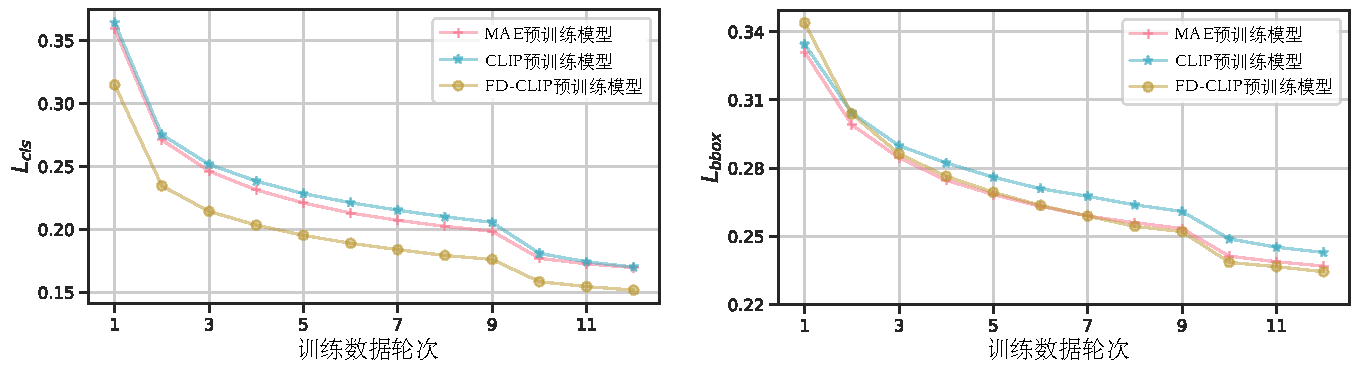
\includegraphics[width=1.0\linewidth]{figures/fd-coco-abl.pdf}
  \caption{MAE、CLIP和FD-CLIP模型在目标检测任务上的损失曲线对比}
    % \todo{图2:在 MSCOCO 对象检测任务上微调 MAE、CLIP 和 FD-CLIP。我们可视化了 $L_{cls}$ 和 $L_{bbox}$ 相对于训练时期的损失曲线。虽然 CLIP 预训练与 $L_{cls}$ 的 MAE 预训练相当,但它显示出更差的定位能力,反映在 $L_{bbox}$ 曲线上。}
    % 还有一个lvis的,可以画在ablation里
  \label{fig:fd-coco-abl}
\end{figure}

% 语言-图像对比学习方法能整合通过对比巨大的图像文本对学到的丰富语义而闻名,与MIM方法(例如MAE)相比,CLIP方法得到的视觉模型与人类概念联系更紧密。然而,它令人印象深刻的语义能力似乎对下游任务微调的好处帮助有限。

本节首先分析了语言-图像对比学习CLIP方法和掩码图像模型MAE方法在MSCOCO\cite{chen2015microsoft}数据集目标检测任务上的表现。
目标检测任务主要包含目标定位与物体识别两个任务\cite{ren2016faster},前者属于需要密集感知能力的细粒度任务,而后者则属于对语义能力要求较高的实例级任务。因此可以观察不同预训练方法的视觉模型在两种不同任务上的行为表现。
图\ref{fig:fd-coco-abl}中展示了不同预训练模型在MSCOCO数据集上的训练损失曲线。在物体识别训练损失$L_{cls}$上,掩码图像模型MAE方法和语言-图像对比学习CLIP方法之间表现非常接近,但掩码图像模型MAE方法预训练的模型则具有更好的细粒度感知能力,因此其目标定位损失$L_{bbox}$相较于语言-图像对比学习CLIP方法得到的模型更低。
这些差异促使本章进一步研究影响CLIP模型迁移性能的关键因素,以更好地释放其预训练中掌握的语义信息,同时增强其处理细粒度视觉任务能力。

\begin{table}
\caption{
不同预训练方法的输入完整性、训练目标粒度和损失函数设计}
% ,除了MAE方法之外,BEiT也是一个典型的像素级自监督预训练方法。
\centering
  \begin{tabular}{lcccc}
    \toprule
  方法 & 输入完整性 & 训练目标粒度 & 损失函数设计 & 是否使用语义信息 \\
  \midrule
  BEiT & 部分图像 & 像素级任务 & 交叉熵损失函数 & \\ 
  MAE & 部分图像 & 像素级任务 & 回归损失函数 & \\
  % SimMIM~\cite{xie2021simmim}? & partial? & token-level & regression & \\ % if we mentioned them, we need to put it in table1?
  \midrule
  CLIP & 完整图像 & 实例级任务 & 交叉熵损失函数 & $\checkmark$  \\
  % 新方法 & Full & Token-level & \color{gray}{Regression} & $\checkmark$ \\
\bottomrule
  \end{tabular}
\label{tab:fd-differences}
\end{table}

% 要回答这个问题,本章首先将这些预训练方法的要素分解为三个方面:输入完整性、训练目标粒度和损失函数设计。
% 如表\ref{tab:fd-differences}所示,通过比较CLIP与两种典型MIM方法之间的设计要素差异,可以排除了损失函数设计为主要影响因素,并推测输入完整性(是否使用对完整图像还是部分图像进行建模)和训练目标粒度(是实例级监督任务还是像素级监督任务)是可能因素。
% 结合自监督预训练任务发展历史上实例级自监督任务与像素级自监督任务的对比\cite{xie2021propagate},像素级训练目标粒度的设计可能对模型在下游任务的迁移效果以及在细粒度视觉任务上的表现起到关键因素。
% 为了验证这两项因素分别对实例级语言监督预训练方法CLIP的模型迁移能力的影响,需要在现有方法中引入相应设计。尽管对齐输入完整性的差异相对简单,但要将CLIP的训练目标的粒度从实例级扩展到像素级是一个重大挑战,因为这种方案不符合大规模互联网数据的基本形态,(图像,替代文本)对往往只反映实例级的对应信息,缺乏对细粒度关系的标注。
% 尽管有一些工作如局部化叙事\cite{LocNar}(Localized Narratives)提出了一些新的相对高效的数据标注方法来引入像素级对齐的信息,但这样的方法的数据可扩展性还是很低,违背了以CLIP为例预训练方法的重要出发点。

为进一步分析,本节将不同预训练方法的核心要素分解为三个方面:输入完整性、训练目标粒度和损失函数设计。表\ref{tab:fd-differences}中展示了语言-图像对比学习方法和两个典型的掩码图像模型MAE与BEiT\cite{bao2021beit}方法之间的设计差异。对比这些差异后可以排除损失函数设计的影响因素,因此本节考虑对齐掩码图像模型方法,使用一致的输入完整性和训练目标粒度设计来增强CLIP模型在下游视觉任务中的迁移性能。
% 并推测输入完整性(是否使用对完整图像还是部分图像进行建模)和训练目标粒度(是实例级监督任务还是像素级监督任务)是可能因素。
% :输入完整性、训练目标粒度和损失函数设计,本节考虑对齐MIM方法设计中使用的输入完整性和训练目标粒度来增强CLIP模型的迁移性能。
在这两个方面中,使用部分图像作为CLIP方法的输入相对容易\cite{FLIP},但将CLIP方法的训练目标粒度从实例级扩展到像素级是一个重大挑战,因为大规模获取图像像素与文本内容细粒度对齐的图文对数据非常困难。此外,CLIP模型预训练过程中使用超过4亿张训练图片和数百张显卡训练数周。由于重新训练成本高昂,本节提出的方法旨在避免重新预训练且不需要额外数据标注的前提下,在语言-图像对比学习方法中引入部分图像的输入设计和像素级的训练目标粒度设计。

\subsection{特征图自蒸馏方法}

\begin{figure}
  \centering
  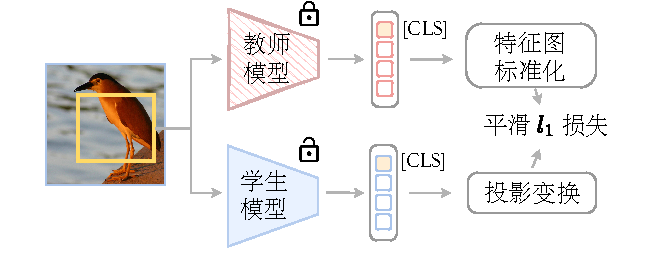
\includegraphics[width=0.8\linewidth]{figures/fd-overall.pdf}
  \caption{利用特征图自蒸馏方法引入像素级训练信号的流程图}
  % \todo{图 1:特征图蒸馏图,引入令牌级目标来蒸馏预训练的 CLIP 模型。橙色块代表 [\texttt{CLS}] 令牌,橙色框表示原始图像的随机裁剪。}
  \label{fig:fd-overall}
\end{figure}

% 整个过程如图\ref{fig:fd-overall}所示,输入图像的黄色框代表对原始图像进行随机裁剪的数据增强方法,输出特征图中的橙色块对应着描述了图像全局信息的特殊标记[\texttt{CLS}]。

% 特征图自蒸馏方法与传统的未归一化概率知识蒸馏的方法\cite{hinton2015knowledge,deit}不同。一方面前者采用特征图作为蒸馏信号,而后者采用模型输出的类别未归一化概率作为蒸馏信号,另一方面前者以引入像素级训练目标为主要目的,需要尽可能保留教师模型能力,因此使用参数量一致的学生模型,而后者则主要被用于模型压缩场景,常使用参数量小得多的学生模型。

受知识蒸馏方法启发,本节提出利用知识蒸馏作为桥梁,将语言-图像对比学习方法的训练目标粒度从实例级扩展到像素级,同时最大程度保留预训练CLIP模型的语义信息。
整个特征图自蒸馏过程如图\ref{fig:fd-overall}所示。输入图像的黄色框代表对原始图像进行随机裁剪的数据增强方法,输出特征图中的橙色块对应着描述了图像全局信息的特殊标记[\texttt{CLS}],这一标记在语言-图像对比学习预训练过程对齐了文本的全局特征。
和传统知识蒸馏方法类似,特征图自蒸馏方法使用预训练完成的CLIP模型充当教师模型并固定参数不动,同时随机初始化一个新模型作为学生模型,来尽可能保留教师模型预训练过程中建模的语义信息。%,同时在此阶段引入像素级任务以增强视觉模型在细粒度任务上的迁移表现。

和传统知识蒸馏方法不同,特征图自蒸馏方法有如下两个特征:
\begin{itemize}
    \item 采用预训练模型的完整输出特征图作为蒸馏目标,而不是以未归一化概率为蒸馏目标\cite{hinton2015knowledge,deit}。一方面这样的做法可以引入像素级训练目标,并为学生模型提供更多可蒸馏信号以尽可能保留教师模型的能力。另一方面这种设计也允许将该方法运用到更多预训练模型中,因为很多预训练模型\cite{dino}并没有未归一化概率作为输出。
    此外,为了确保特征图逐像素对齐,特征图自蒸馏方法需要对输入教师模型和学生模型的图像应用相同的图像增强方法。
    后续实验表明,与蒸馏其他实例级特征相比,蒸馏整个特征图可以更显著地增强CLIP模型在下游视觉任务的微调效果,验证了之前关于像素级训练目标对模型细粒度视觉任务微调效果重要性的猜想。
    \item 使用相同大小的教师模型和学生模型,而不是大参数的教师模型和小参数的学生模型。因为特征图自蒸馏方法并非为了压缩模型,而是为了在引入像素级训练目标的同时,尽可能使得学生模型保留教师模型中蕴含的语义信息和视觉能力。
    虽然学生模型的训练目标是尽可能模仿教师模型的输出特征图,但从随机初始化开始训练允许学生模型有不同的优化路径。这种优化路径上的差异为学生模型提供了与掩码图像模型具有相似特征属性的可能性。
\end{itemize}

% \begin{figure}
%   \centering
%   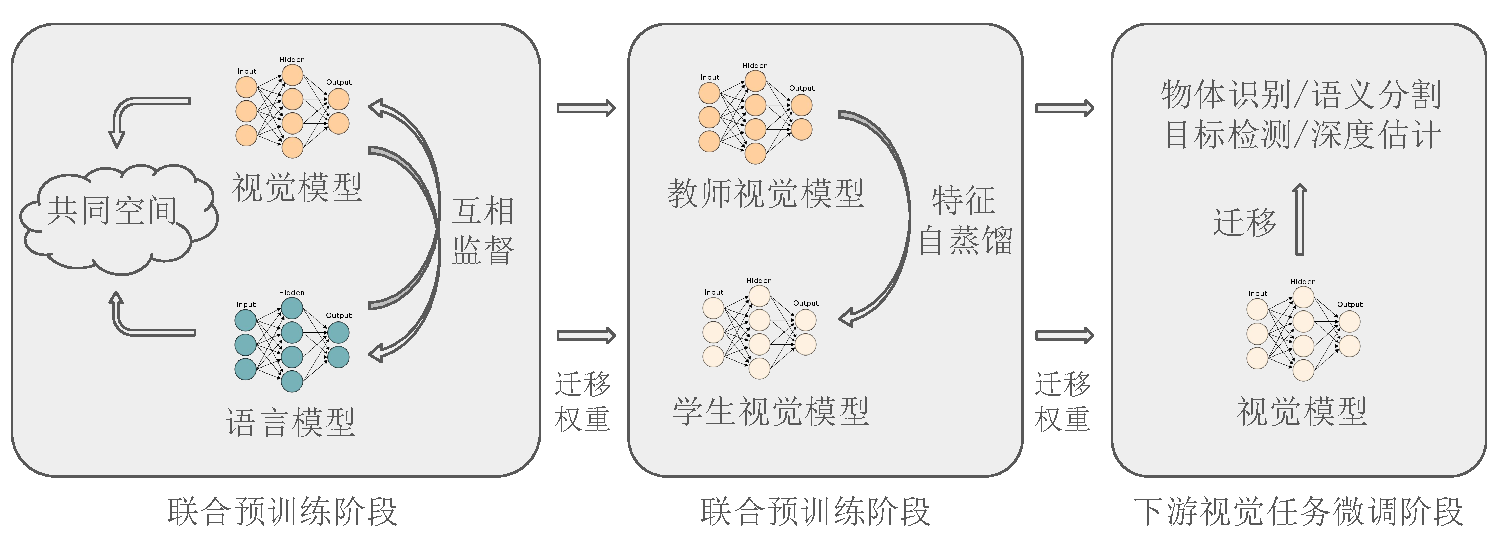
\includegraphics[width=1.0\linewidth]{figures/fd-framework-update.pdf}
%   \caption{新引入的“特征图自蒸馏”阶段在整个“预训练-微调”范式中的作用}
%     % \todo{图2:在 MSCOCO 对象检测任务上微调 MAE、CLIP 和 FD-CLIP。我们可视化了 $L_{cls}$ 和 $L_{bbox}$ 相对于训练时期的损失曲线。虽然 CLIP 预训练与 $L_{cls}$ 的 MAE 预训练相当,但它显示出更差的定位能力,反映在 $L_{bbox}$ 曲线上。}
%   \label{fig:fd-framework-update}
% \end{figure}

\begin{table}
\caption{特征图自蒸馏方法为语言-图像对比学习方法提供像素级训练目标}
\centering
  \begin{tabular}{lcccc}
\toprule
  方法 & 输入完整性 & 训练目标粒度 & 损失函数设计 & 是否带语义信息 \\
  \midrule
  MAE & 部分图像 & 像素级任务 & 回归损失函数 & \\
  % SimMIM~\cite{xie2021simmim}? & partial? & token-level & regression & \\ % if we mentioned them, we need to put it in table1?
  \midrule
  CLIP & 完整图像 & 实例级任务 & 交叉熵损失函数 & $\checkmark$  \\
  FD-CLIP & 完整图像 & 像素级任务 & 回归损失函数 & $\checkmark$ \\
\bottomrule
  \end{tabular}
\label{tab:fd-method}
\end{table}

% 因此,该方法称作“特征图自蒸馏”方法,因其使用的蒸馏目标是特征图,教师模型是它自身。
如表\ref{tab:fd-method}所示,通过以上设计,特征图自蒸馏方法得以在保留CLIP模型语义信息的同时,不需要额外数据标注即可引入像素级训练信号,从而达到以较小的代价增强CLIP模型在下游视觉任务迁移性能的目的。% 新引入的“特征图自蒸馏”方法在整个“预训练-微调”范式中xxx。该阶段在不重新预训练CLIP模型的前提下,以较小的成本引入像素级监督任务,可以理解为是针对预训练模型的一次“中间训练”(Mid-training)。

\subsection{归纳偏置和正则化方法设计}
基于特征图自蒸馏方法的双分支结构,本节提出在蒸馏过程中引入额外的归纳偏置和正则化方法,以进一步提升学生模型在下游视觉任务上的迁移性能。
% 接着,在“特征图自蒸馏”方法基础上,本节设计并引入以下归纳偏置和正则化策略,以进一步提高学生模型的迁移效果。
\paragraph{对教师模型的输出特征图进行标准化} 不同预训练模型的输出特征图有各自的数值范围,直接回归这些特征图使得蒸馏过程中需要针对不同模型调整超参数,限制了方法的通用性。此外,一些特征图中的细节信息被编码在相对小的数值中。如果不对这些细微信号进行放大,学生模型在蒸馏过程中往往会忽略这些信息。为了解决这些问题,本节提出使用标准化操作对教师网络的输出特征图进行后处理,使得不同输出特征图的均值为0,方差为1。% https://ssjcoding.github.io/2019/03/27/normalization-and-standardization/
该操作可通过五参数的层归一化\cite{ba2016layer}实现。接着,特征图自蒸馏方法在学生和教师模型特征图之间采用平滑$\ell_{1}$损失函数进行监督,以减少离异特征值的影响。% https://blog.csdn.net/ai_faker/article/details/117414614
以$s$和$t$分别表示学生和教师模型的输出特征图,特征图自蒸馏方法公式化如下:
\begin{equation}
    \mathcal{L} (s, t) = \begin{cases}
        \frac{1}{2} (g(s) - t')^2/\beta, & | g(s) - t' | \leq \beta \\
        |g(s)-t'|-\frac{1}{2}\beta, & | g(s) - t' | > \beta,
    \end{cases}
    \label{eq:iclip-distill}
\end{equation}
其中$\beta$值设为2,而$t'$表示对教师输出特征图$t$进行标准化后的特征图。$g$是单个线性层,实现轻量级的投影变换以允许教师和学生模型之间有不同的输出特征图维度,从而增强了该方法的通用性。此外,考虑到在语言-图像对比学习训练过程中,CLIP模型通过特殊标记[\texttt{CLS}]聚合图像全局信息并与语言表征进行对齐,因此[\texttt{CLS}]标记相比于特征图中的其他位置蕴含了更丰富的语义信息。在特征图自蒸馏方法中,[\texttt{CLS}]标记对应的蒸馏损失权重为其他位置的10倍,从而增强学生模型保留教师模型语义信息的效果。

\paragraph{不对称比例的随机深度} 特征图自蒸馏方法的双分支结构允许在教师模型和学生模型上应用不对称的正则化强度。实验发现,这种策略可以使学生模型在下游视觉任务的迁移性能更佳。具体来说,特征图自蒸馏过程中会在学生模型分支上添加一定比例的随机深度正则化,而在教师模型分支上不添加任何正则化。这种设计既保证了教师模型的蒸馏信号稳定性,不对学生模型的训练造成干扰,又减轻了学生模型的过拟合风险。

\paragraph{层间共享的相对位置偏置} 原始的CLIP模型采用绝对位置编码策略,也即通过对不同位置的输入标记使用不同的索引来进行区分。最近的工作\cite{Swin,li2022mvitv2}发现相对位置偏置增强了图像表征的平移不变性,因此对模型的迁移性能有一定好处。
由于特征图自蒸馏方法只依赖模型最后一层特征图,因此可以调整学生模型的位置编码策略。实验表明层间共享的相对位置偏置策略\cite{bao2021beit}能够提升模型的迁移性能。因为这种策略要求模型的所有层使用相同的相对位置偏置矩阵,可以在一定程度上避免较深的模型层因为不同位置间的特征过于相似而出现表征坍缩的问题\cite{xie2023revealing}。% 实验表明,层间共享的相对位置偏置的总体性能最佳。
通过模型特征属性诊断工具可以发现使用这种位置编码策略使得模型不同注意力头的感受野更加多样化,允许模型建模局部或全局更多不同的图像信息。这一现象在更深的模型层中较为明显。% (\todo{如补充材料中的图所示})

\subsection{模型特征属性的诊断工具}
为进一步理解特征图自蒸馏前后模型行为的变化,本节引入多个特征属性诊断工具对不同的模型进行对比分析,以提供对特征图自蒸馏方法背后机制的直观理解:
\begin{itemize}
    \item 注意力头级别的诊断工具:平均注意力距离\cite{dosovitskiy2020vit,xie2023revealing}。本文使用的视觉模型架构为视觉Transformer,简称为ViT\cite{dosovitskiy2020vit}。ViT结构中的自注意力层建模了不同像素位置间的相关关系,而每个自注意力层包含多个自注意力头用于建模不同的像素间关系。平均注意力距离的诊断工具统计了每个像素与其他像素间经过注意力权重加权后的相对距离的平均值,因此反映了每个自注意力头的感受野范围大小。在统计过程中,由于特殊标记[\texttt{CLS}]不包含任何位置信息,因此不会纳入统计范围。
    \item 模型层级别的诊断工具:平均注意力图\cite{zhou2021deepvit}。通过平均所有注意力头的注意力图可以得到层级别的平均注意力图。注意力图中有两种常见的模式:对角线模式和竖线模式。对角线模式表明该模型更多地依赖于来自相对位置关系的视觉线索,具有更好的图像表征平移不变性,这是对各种下游视觉任务迁移性能的有益属性。同时,越是靠近中心对角线的对角线模式越能反映出模型学到了一些基于图像连续性的局部先验。而竖线模式则表明处于某些固定位置的图像输入对所有其他位置的特征产生了较大影响,这种模式反映了模型提取的图像表征往往是平移变化的,抗干扰能力较弱。
    \item 模型级别的诊断工具:归一化的损失景观\cite{li2018visualizing}。这一诊断工具通过对微调后的模型权重施加一系列不同程度的高斯噪声进行扰动,并观察扰动后的模型性能变化。噪声强度根据每个权重的$\ell_2$范数来决定,以消除不同模型权重幅度不同的影响。通常而言,在微调损失局部极小值附近较平坦的损失景观反映了模型更低的测试误差和更好的泛化能力。
\end{itemize}

\section{实验结果}
\label{sec:fd-result}

% 本节展示了在已经训好的CLIP模型基础之上引入特征图自蒸馏阶段对下游任务迁移性能的提升情况,并对该方法的一些关键设计、推广性和诊断性质进行了深入分析。
第\ref{sec:fd-exp-setting}节介绍了特征图自蒸馏阶段和后续视觉任务微调的实验设置。第\ref{sec:fd-exp-clip}节中展示了特征图自蒸馏后的CLIP模型在各类下游视觉任务的性能提升情况,并在第\ref{sec:fd-exp-input}节讨论了输入图像完整性和不同训练目标粒度的影响。第\ref{sec:fd-exp-detail}节包含归纳偏置和正则化设计影响的消融实验,并在第\ref{sec:fd-more-models}节展示了将特征图自蒸馏方法应用到其他预训练模型后对下游任务迁移性能的提升情况。
最后,在第\ref{sec:fd-analysis}节中运用模型特征属性的诊断工具对蒸馏前后的模型进行了分析,深入理解该方法特性。

\subsection{实验设置}
\label{sec:fd-exp-setting}
\paragraph{蒸馏阶段实验设置} 所有实验均使用ImageNet-1K\cite{deng2009imagenet}训练图像进行特征图自蒸馏。特征图自蒸馏方法以教师模型的输出特征图为监督目标,不依赖图像类别等人工标注信息,因此也可以在别的图像数据集上进行应用。除非特别说明,所有实验都在ImageNet-1K数据集(缩写为IN-1K)上蒸馏了100轮次,并默认使用ViT-Base\cite{dosovitskiy2020vit}结构的CLIP模型进行实验(缩写为CLIP-Base)。%\todo{其他详细信息在补充材料中。}
\paragraph{微调阶段实验设置} 为充分评测模型在各类下游视觉任务上的微调效果,本节选择了4个下游任务:ImageNet-1K数据集\cite{deng2009imagenet}上的图像分类任务、ADE20K数据集\cite{zhou2019ade}上的语义分割任务、MSCOCO数据集\cite{chen2015microsoft}上的目标检测和实例分割任务以及NYUv2\cite{NYUv2}数据集上的深度估计任务。除图像分类任务外,其余三项任务均为细粒度视觉任务。各任务的具体设置如下:
\begin{itemize}
    \item \textbf{图像分类任务}~~ 该任务的微调方法按照BEiT\cite{bao2021beit}方法的设置,使用AdamW优化器\cite{adamw}、逐层衰减的学习率和$224 \times 224$的输入图像分辨率。CLIP-Base模型在该任务上微调100轮次,而CLIP-Large模型则微调50轮次。线性探测微调实验则按照MAE方法的设置,使用LARS优化器\cite{lars}和0.1的学习率,并将权重衰减设置为0,共训练90轮次。最终报告ImageNet-1K评测集上的Top-1准确率。
    \item \textbf{语义分割任务}~~  该任务按照Swin\cite{Swin}方法中的描述,使用常用的UPerNet框架\cite{xiao2018upernet}进行微调。微调时使用AdamW优化器,以32的批大小训练8万个数据批次。其他超参数设置:学习率为4e-4、学习率逐层衰减强度为0.65、权重衰减为0.05、随机深度比例为0.2。在训练中,输入图像分辨率设置为$512 \times 512$。在评测中使用单尺度输入进行测试并报告模型在验证集上的mIoU得分。
    \item \textbf{目标检测和实例分割任务}~~  该任务微调阶段采用常见方法\cite{cae}的设置,包括使用MaskRCNN框架\cite{Mask-rcnn}训练12轮次,并使用多尺度训练和单尺度测试策略。为了降低全局自注意力层在高分辨率图像上的训练代价和内存开销,在该任务微调时采用了滑动窗口注意力机制\cite{Swin},并将窗口的像素大小设置为$224 \times 224$,使其与预训练和蒸馏阶段中使用的图像尺寸一致。为了聚合图像的全局信息,在模型最后添加了一个额外的全局自注意力层。其他超参数设置如下:微调过程中的批大小为16、最大学习率为2e-4、学习率逐层衰减系数为0.75,并遵循惯例,在第9和第11轮将学习率降低至先前的0.1倍。最终报告模型在开发集上的检测框mAP和分割掩码mAP得分。
    \item \textbf{深度估计任务}~~  该任务的微调阶段采用已有工作\cite{glpdepth, xie2023revealing}的设置,使用其中的24000张图像作为训练集微调25轮次,并在包含654张图像的官方测试集上进行评测,共涵盖了215个不同室内场景的深度估计任务。其他超参数设置如下:输入图像被随机裁剪为$480 \times 480$的分辨率、微调过程中的批大小为24、学习率为5e-5。该任务的微调框架和数据增强方案沿用已有工作\cite{xie2023revealing},并在测试时平均了两个方形窗口的预测结果。最终报告模型在评测集上的均方根误差(RMSE)。
\end{itemize}

\paragraph{蒸馏阶段和微调阶段的超参数设置}
表\ref{tab:fd-hyper-pretrain}中详细描述了蒸馏阶段和图像分类任务微调阶段的超参数设置。

\begin{table}
    \centering
    \caption{特征图自蒸馏方法在蒸馏阶段和微调阶段的超参数设置}
    \begin{tabular}{lcccc}
    \toprule
        & \multicolumn{2}{c}{蒸馏阶段} & \multicolumn{2}{c}{微调阶段} \\
        \bf 超参数名称 & \bf CLIP-Base & \bf CLIP-Large & \bf CLIP-Base & \bf CLIP-Large \\
        \midrule
            图像块大小 & $16 \times 16$ & $14 \times 14$ & $16 \times 16$ & $14 \times 14$ \\
            层数  & 12 & 24 & 12 & 24\\
            隐变量维度 & 768 & 1024 & 768 & 1024\\
            前馈层中间维度 & 3072 & 4096 & 3072 & 4096 \\
            注意力头数目 & 12 & 16 & 12 & 16 \\
            注意头宽度 & 64 & 64 & 64 & 64 \\
        \midrule
            训练轮次 & 300 & 300 & 100 & 50 \\
            批大小 & 2048 & 2048 & 2048 & 2048  \\
            输入图像分辨率 & $224 \times 224$& $224 \times 224$& $224 \times 224$& $224 \times 224$\\
            优化器参数$(\epsilon)$ & 1e-8 & 1e-8 & 1e-8 & 1e-8  \\
            优化器参数$(\beta)$ & (0.9,0.999)& (0.9,0.999)& (0.9,0.999)& (0.9,0.999)  \\
            最大学习率 & 1.2e-3 & 1.2e-3 & \{5e-3,6e-3\} & 1e-3  \\
            最小学习率 & 2e-5 & 2e-5 & 2e-6 & 2e-6 \\
            学习率调度形式 & 余弦调度 & 余弦调度 & 余弦调度 & 余弦调度 \\
            学习率热启动轮 & 10 & 10 & 20 & 5 \\
            学习率衰减系数 & 1.0 & 1.0 & \{0.6,0.65\} & 0.75 \\
        \midrule
            梯度截断系数 & 3.0 & 3.0 & 5.0 & 5.0 \\
            % Dropout & \multicolumn{4}{c}{\xmark} \\
            权重衰减系数 & 0.05 & 0.05 & 0.05 & 0.05\\
            随机深度比例 & 0.1 & 0.3 & \{0.1,0.2,0.3\} & 0.4 \\
            标签平滑比例 & - & - & 0.1 & 0.1 \\
            % 数据增强方法 & \multicolumn{2}{c}{随机缩放裁剪} & \multicolumn{2}{c}{ }\\
            % 这个列起来好长啊。。。
        \bottomrule
    \end{tabular}
    \label{tab:fd-hyper-pretrain}
\end{table}

\subsection{特征图自蒸馏后的CLIP模型迁移效果}
\label{sec:fd-exp-clip}
\paragraph{特征图自蒸馏后的CLIP-Base模型迁移效果} 本节首先在CLIP-Base模型上进行特征图自蒸馏实验,并将数据轮次扩展到300轮次以充分验证结果。表\ref{tab:fd-clip_FD}展示了特征图自蒸馏后的模型在各类下游视觉任务上的微调表现。
经过特征图自蒸馏后得到的FD-CLIP模型在各类下游视觉任务上都有一定的性能提升,并在一些细粒度视觉任务上提升更为显著。相比于原始CLIP模型,FD-CLIP模型在ImageNet-1K图像分类任务上提高2.1\%的Top-1准确率,在图像语义分割任务上提高了2.2的mIoU得分,并在目标检测和实例分割任务上分别改善了3.2和2.7的检测框mAP和分割掩码mAP得分。此外,FD-CLIP模型在深度估计任务上也取得了明显的提升,均方根误差从0.416降低到了0.352。与此同时,FD-CLIP模型在各类下游视觉任务上的微调表现已经超过了掩码图像模型MAE方法,验证了特征图自蒸馏能够显著提升语言-图像对比学习方法在下游视觉任务上的迁移性能。

\begin{table}
\caption{特征图自蒸馏前后的CLIP-Base模型在下游视觉任务上的效果对比
% 该模型是在 ImageNet-1K 数据集 [10] 上提炼的,其中的图像只有 300 个 epoch。在四个评估基准上观察到明显的进步。MAE [17] 结果也以灰色列出以供参考。
}
\centering
% \addtolength{\tabcolsep}{-3.0pt}
% \renewcommand{\arraystretch}{1.1}
  \begin{tabular}{lccccc}
\toprule
   & IN-1K & ADE20K & \multicolumn{2}{c}{MSCOCO} & NYUv2 \\
   % \cline{2-3} \cline{5-6}
   \midrule
   % {AP$_\text{box}$} & {AP$_\text{mask}$}
方法    &   Top-1准确率 &  mIoU  & 检测框mAP & 分割掩码mAP & RMSE\scriptsize{ ($\downarrow$)}\\
  \midrule
  MAE & 83.6 & 48.1 & 46.5 & 40.9 & 0.383 \\

  \midrule
  
  CLIP & 82.9  & 49.5 & 45.0 & 39.8 & 0.416 \\
  FD-CLIP & 85.0  & 51.7 & 48.2 & 42.5 & 0.352 \\
  $\Delta$ & \textbf{$\uparrow$2.1}  &  \textbf{$\uparrow$2.2} & \textbf{$\uparrow$3.2} & \textbf{$\uparrow$2.7} & \textbf{$\downarrow$0.064}\\
\bottomrule
  \end{tabular}
\label{tab:fd-clip_FD}
\end{table}

% 在其他Validation set上的评测,表示健壮性
% To further evaluate the robustness of our model, we include more adversarial validation sets. Our FD-CLIP reaches 75.0\% and 43.8\% top-1 accuracy on ImageNet-v2 and ImageNet-sketch, higher than the original CLIP by \textbf{2.5\%} and \textbf{10.6\%}, respectively. These results show our method is not overfitted on ImageNet-1k validation set.

\begin{table}
\caption{特征图自蒸馏后的模型在零样本和线性探测任务上的表现
% \yx{Put init weight to appendix.} [这个啥意思来着?]
}
% \vspace{-0.3em}
\centering
% \addtolength{\tabcolsep}{-1.5pt}
% \renewcommand{\arraystretch}{1.1}
  \begin{tabular}{lccc}
\toprule
  评测方法 & CLIP & FD-CLIP & $\Delta$ \\
  \midrule
  零样本图像识别任务 (Top-1准确率) & 68.6 & 68.0 & -0.6 \\
  线性探测图像识别任务 (Top-1准确率) & 79.5 & 80.1 & +0.6 \\ 
\bottomrule
  \end{tabular}
\label{tab:fd-zero_shot}
\end{table}

\paragraph{特征图自蒸馏后的模型对预训练语义信息的保留情况} 
尽管特征图自蒸馏方法的训练目标与原始语言-图像对比学习训练目标不同,但因为蒸馏过程中学生模型充分学习了教师模型特征图,因此学生模型保留了大部分语义信息。
表\ref{tab:fd-zero_shot}比较了蒸馏前后的教师模型与学生模型在ImageNet-1K评测集上零样本和线性探测图像识别任务的Top-1准确率。结果表明蒸馏后的学生模型保留了原始CLIP模型蕴含的大部分语义信息。
% 也就是说,基于完整特征图的特征图自蒸馏方法可以在很大程度上保留了CLIP模型中包含的大量语义信息,同时可以取得优于MIM方法的迁移性能。

\paragraph{特征图自蒸馏方法的额外训练代价} 前述特征图自蒸馏方法使用ImageNet-1k数据集训练了300轮次,而ImageNet-1K数据集包含128万张图像,因此总训练图像数目约为3.84亿张。原始CLIP模型预训练阶段使用私有的WIT-400M图文对数据集\cite{radford2021learning}训练了32轮次,其中包含4亿张图片,因此总训练图像数目约为128亿张。由于语言模型参数量远小于视觉模型,此处忽略其预训练成本。
因此,特征图自蒸馏方法通过3\%的可控额外训练成本,无须重新预训练或额外数据标注,即可在各类下游视觉任务上带来大幅度性能提升。
% 这个代价是可以接受的,而且该方法不需要对CLIP进行重新训练,也不需要引入额外的数据标注代价。
此外,CLIP预训练过程依赖大量显卡组成的集群才能达到足够的批大小。原始CLIP模型需要256张以上显卡同时训练,而特征图自蒸馏方法对硬件要求较低,应用更为灵活。%对大多数实验室和团队都更友好。
% 原始的CLIP模型使用32768 的批大小和256个GPU进行训练,与CLIP预训练不同,特征图自蒸馏方法仅需要更小的批大小(2048),且只需要8个GPU即可训练,这对大多数实验室和团队都更友好。


\begin{table}
\caption{
特征图自蒸馏前后的CLIP-Large模型在图像分类任务的效果对比
% 扩展特征图自蒸馏方法至CLIP-Large模型后在图像任务上的迁移性能
}
\centering
% \addtolength{\tabcolsep}{-1.0pt}
% \renewcommand{\arraystretch}{1.1}
  \begin{tabular}{lccc}
\toprule
 方法 & 图像分辨率 & 训练数据集 & IN-1K Top-1准确率 \\
  \midrule
    WiSE-FT~\cite{ftclip2021} & 336$^2$ & WIT-400M~\cite{radford2021learning} & 87.1 \\
    DeiT III~\cite{touvron2022deit} & 384$^2$ & IN-22K~\cite{deng2009imagenet} & 87.7 \\
    ViT~\cite{dosovitskiy2020vit} & 512$^2$ & JFT-300M~\cite{Sun_2017_JFT300m} & 87.8 \\
   Scaling~\cite{zhai2022scaling} &  384$^2$ &  JFT-3B\cite{zhai2022scaling} &  88.5 \\
   BEiT~\cite{bao2021beit} &  512$^2$ &  DALLE~\cite{ramesh2021dalle1} \& IN-22K &  88.6 \\

  \midrule
  CLIP & $224^2$ & WIT-400M & 86.1 \\
  \midrule
  \multirow{3}{*}{FD-CLIP} & $224^2$ & WIT-400M & \textbf{87.7}\scriptsize{ (+1.6)} \\
   & 224$^2$ & WIT-400M \& IN-22K & \textbf{88.3}\scriptsize{ (+2.2)} \\
   & 336$^2$ & WIT-400M \& IN-22K & \textbf{89.0}\scriptsize{ (+2.9)} \\
\bottomrule
  \end{tabular}
\label{tab:fd-clip_large_FD}
\end{table}

\paragraph{特征图自蒸馏后的CLIP-Large模型微调效果} 本组实验将特征图自蒸馏方法应用于CLIP-Large模型,验证该方法的可扩展性。
如表\ref{tab:fd-clip_large_FD}所示,经过特征图自蒸馏后的FD-CLIP模型在ImageNet-1K数据集图像分类任务中取得了87.7\%的Top-1准确率,相比原始CLIP模型提升1.6\%。
使用ImageNet-22K数据集微调,并将图像分辨率扩展至$336\times 336$后,FD-CLIP模型在图像分类任务上取得了89.0\%的Top-1准确率,超过了使用接近10倍多预训练数据方法\cite{zhai2022scaling}的性能表现。% 因为CLIP-Large模型使用14的块大小,并非2的整次幂,多分辨率的FPN与模型的块大小不兼容,因此没有在其他下游任务上进行微调比较。

\subsection{训练目标粒度和输入完整性对迁移性能的影响}
\label{sec:fd-exp-input}

\paragraph{训练目标粒度对迁移性能的影响} 本组实验研究了不同训练目标粒度对下游任务迁移性能的影响。本组实验比较了三种不同的训练目标粒度设置:
\begin{itemize}
    \item \textbf{蒸馏特殊标记特征}~~ 视觉模型中的[\texttt{CLS}]标记是一个特殊标记,并在CLIP模型中起到独特的作用:它不仅聚合了全局的图像信息,而且直接与语言表征进行对齐,因此蕴含了丰富的语义信息。在此设置中,蒸馏过程以教师模型的[\texttt{CLS}]标记输出特征作为训练目标构建了实例级训练目标粒度。
    \item \textbf{蒸馏全局平均特征}~~ 此设置是介于实例级训练目标粒度和像素级训练目标粒度的中间形式。具体来说,此设置对教师模型的输出特征图应用全局平均操作,以构造一个简化后的蒸馏目标。因此这个蒸馏目标同时包含了来自每个像素的特征信息,但又缺乏像素级的训练目标分辨率。
    \item \textbf{蒸馏完整特征图}~~ 这是特征图自蒸馏方法的默认设置,使用了教师模型的完整输出特征图作为蒸馏目标来构建像素级的训练目标粒度,并对[\texttt{CLS}]标记的对应特征使用更大的损失权重。
\end{itemize}

\begin{table}
\caption{FD-CLIP使用不同训练目标粒度的消融实验}
% 。这些模型是在 ImageNet-1K 数据集 [10] 上蒸馏的,有 100 个 epoch。代币级目标对于提高 CLIP 的迁移性能至关重要。
\centering
% \addtolength{\tabcolsep}{-2.5pt}
% \renewcommand{\arraystretch}{1.1}
  \begin{tabular}{lccccc}
\toprule
   & IN-1K & ADE20K & \multicolumn{2}{c}{MSCOCO} & NYUv2 \\
   % \cline{4-5}
   \midrule

   方法 &  Top-1准确率   &  mIoU  & 检测框mAP & 分割掩码mAP & RMSE\scriptsize{ ($\downarrow$)}\\
  \midrule

  MAE & 83.6 & 48.1 & 46.5 & 40.9 & 0.383 \\
    原始模型 & 82.9 & 49.5 & 45.0 & 39.8 & 0.416 \\ 
  % CLIP~\cite{radford2021learning} & 82.9 & 49.5 & 45.0 & 39.8 & 0.416 \\
  \midrule
  % FIXME: 这个要修-编译bug
  特殊标记特征 & 81.9 & 47.5 & 44.8 & 39.6 & 0.396 \\
  全局平均特征  & 83.3 & 50.3 & 46.3 & 40.6 & 0.393 \\
  完整特征图 & \textbf{84.4} & \textbf{51.8} & \textbf{47.9} & \textbf{42.2} & \textbf{0.350} \\
\bottomrule
  \end{tabular}
\label{tab:fd-ablation_targets}
\end{table}

表\ref{tab:fd-ablation_targets}展示了通过不同训练目标粒度蒸馏后的模型在下游任务上的迁移性能表现。蒸馏[\texttt{CLS}]标记特征的模型在深度估计任务上的误差有所减少,但在其他视觉任务上的性能相比原始CLIP模型没有提升,甚至有一定损失。这是因为[\texttt{CLS}]标记无法提供教师模型蕴含的全部信息。相比之下,蒸馏全局平均特征的模型在所有下游视觉任务中均展现出了一定的性能增益,但提升幅度微弱。蒸馏完整特征图的特征图自蒸馏方法引入了像素级训练目标粒度,相比于其他蒸馏目标而言,这一方法得到的模型在下游视觉任务中的微调表现最佳,超过了掩码图像模型MAE方法的微调效果。结果表明像素级训练目标对提升CLIP模型的下游任务迁移性能至关重要。

\paragraph{输入完整性对迁移性能的影响} 这组实验研究了特征图自蒸馏方法中的输入完整性对下游视觉任务迁移性能的影响。为构造不同的输入图像比例,本组实验参考掩码图像模型方法,以块形状随机掩码部分图像后输入模型。%,比例分别设置为25\%、50\%、75\%和100\%(即完整图像)。
表\ref{tab:fd-ablation_masking}展示了对学生模型应用不同输入比例进行自蒸馏后在各类下游任务上的迁移性能,其中标注$^{\dag}$的实验表明教师模型的输入图像也缩减到对应比例,否则教师模型默认使用完整图像作为输入。

在相同的训练轮次下,使用完整图像和部分图像进行特征图自蒸馏得到的模型性能相近,但使用25\%输入比例设置的模型表现不佳。同时,教师模型的输入需要是完整图像,否则自蒸馏后的模型在一些深度估计等任务上的迁移表现欠佳。结果表明输入完整性不是影响CLIP模型在下游视觉任务上迁移效果的关键因素。
\begin{table}
\caption{FD-CLIP使用不同输入比例的消融实验
}
\centering
% \addtolength{\tabcolsep}{-1.5pt}
% \renewcommand{\arraystretch}{1.1}
  \begin{tabular}{lccccc}
\toprule
   & IN-1K & ADE20K & \multicolumn{2}{c}{MSCOCO} & NYUv2 \\
   % \cline{4-5}

   \midrule

   方法  &  Top-1准确率   &  mIoU  & 检测框mAP & 分割掩码mAP & RMSE\scriptsize{ ($\downarrow$)}\\
  \midrule

    MAE & 83.6 & 48.1 & 46.5 & 40.9 & 0.383 \\
    原始模型 & 82.9 & 49.5 & 45.0 & 39.8 & 0.416 \\ 
  % CLIP~\cite{radford2021learning} & 82.9 & 49.5 & 45.0 & 39.8 & 0.416 \\
\midrule
  $25\%$ 输入图像$^{\dag}$ & 83.3 & 47.8 & 45.2 & 40.1 & 0.397 \\
  $25\%$ 输入图像 & 83.1 & 48.8 & 45.1& 39.8& 0.379 \\
  $50\%$ 输入图像 & 84.2 & 51.5 & 47.5& 41.7& 0.351 \\
  $75\%$ 输入图像 & \textbf{84.4} & \textbf{52.0} & 47.8& 41.9 & \textbf{0.347} \\
  完整输入图像 & \textbf{84.4} & 51.8 & \textbf{47.9} & \textbf{42.2} & 0.350 \\
\bottomrule
  \end{tabular}
\label{tab:fd-ablation_masking}
\end{table}

\begin{table}
        \centering
        \caption{使用部分比例输入图像并增加训练轮次的消融实验}
    \
        \begin{tabular}{lccccc}
            \toprule
               & 显卡 & IN-1K & ADE20K & MSCOCO & NYUv2 \\
               %\cline{5-6}
                \midrule
               方法 & 小时 &  Top-1准确率   &  mIoU  & 检测框mAP & RMSE\scriptsize{ ($\downarrow$)}\\
              \midrule
            %   100数据轮次 & 96.4 & 83.1 & 48.8 & 45.1& 39.8& 0.379 \\
            %   200数据轮次 & 192.8 & 83.9 & 49.7 & 46.4& 40.9& 0.366 \\
            %   400数据轮次 & 385.6 & \textbf{84.4} & 51.1 & 47.2& 41.5& 0.367 \\
            % %   $50\%$ + 100ep input & 84.2 & 51.5 & 47.5& 41.7& 0.351 \\
            % %   $50\%$ + 200ep input & 84.6 & 51.5 & 48.3& 42.3& 0.349 \\
            %   100数据轮次$^{\dag}$ & 170.7 & \textbf{84.4} & \textbf{51.8} & \textbf{47.9} & \textbf{42.2} & \textbf{0.350} \\
              100轮次 & 96.4 & 83.1 & 48.8 & 45.1&  0.379 \\
              200轮次 & 192.8 & 83.9 & 49.7 & 46.4& 0.366 \\
              400轮次 & 385.6 & \textbf{84.4} & 51.1 & 47.2&  0.367 \\
            %   $50\%$ + 100ep input & 84.2 & 51.5 & 47.5& 41.7& 0.351 \\
            %   $50\%$ + 200ep input & 84.6 & 51.5 & 48.3& 42.3& 0.349 \\
              100轮次$^{\dag}$ & 170.7 & \textbf{84.4} & \textbf{51.8} & \textbf{47.9} & \textbf{0.350} \\
            \bottomrule
        \end{tabular}
        \label{tab:fd-ablate_longer_maskinput}
\end{table}

考虑到使用25\%输入比例时,特征图自蒸馏方法的计算量相比于蒸馏完整输入图像时要更小,因此表\ref{tab:fd-ablate_longer_maskinput}研究了增加蒸馏训练轮次的影响,其中标注$^{\dag}$的实验代表蒸馏完整输入图像的实验基线。
实验结果表明,延长使用25\%输入比例的蒸馏数据至4倍训练轮次后,模型在细粒度视觉任务上微调表现仍落后于蒸馏完整输入图像的默认设置。考虑到教师模型没法利用部分图像输入进行加速,此时实验设置需要的计算代价已经超过默认设置。因此使用完整输入图像进行蒸馏可以取得更优的微调结果。
此外,表\ref{tab:fd-ablation_masking}的实验结果表明,使用75\%的输入比例进行特征图自蒸馏可以获得相近的迁移性能。此时对图像进行掩码可以被认为是一种数据增强方法,在减少过拟合风险的同时提供一定比例的加速效果。
% 综合以上实验可以得出结论:训练目标粒度对于提升下游视觉任务的迁移性能非常重要,输入完整性的影响不大。


\begin{table}
    % \small
    \centering
    % \renewcommand{\arraystretch}{1.15}
    % \addtolength{\tabcolsep}{-3.5pt}
    \caption{
    特征图自蒸馏中归纳偏置和正则化设计的消融实验}
    \begin{tabular}{lccc}
        \toprule
        (a)特征图后处理设计 & 无 & $\ell_2$ 归一化 & 标准化 \\
        \midrule
        IN-1K (Top-1 准确率) & 83.5 & 83.9 & \textbf{84.4} \\
        \midrule
        (b)学生/教师的随机深度比例 & 0.1 / 0.1 & 0.1 / 0 & 0.2 / 0  \\
        \midrule
        IN-1K (Top-1 准确率) & 84.0 & \textbf{84.4} & 84.0 \\
        \midrule
        (c)位置编码设计 & 绝对位置编码 & 不共享相对编码 & 共享相对编码 \\
        \midrule
        IN-1K (Top-1 准确率) & 84.0 & 83.9 & \textbf{84.4} \\
        \bottomrule
    \end{tabular}
    \label{tab:fd-ablation_tricks}
\end{table}

\subsection{归纳偏置和正则化设计的消融}
\label{sec:fd-exp-detail}
本节讨论了特征图自蒸馏方法中不同归纳偏置和正则化设计对下游任务迁移性能的影响。本节实验对比了不同模型在ImageNet-1K图像分类任务上的微调效果。

\paragraph{不同教师特征图后处理方式的设计} 表\ref{tab:fd-ablation_tricks} (a)中对比了不同教师特征图后处理方式等效果。
与直接使用原始教师模型特征图作为蒸馏信号相比,教师模型特征图标准化带来了0.9\%的Top-1准确率提升。进一步对比$\ell_{2}$归一化方法和标准化方法,后者仍有0.5\%的增益。这种后处理方法使得特征图自蒸馏阶段的超参数对使用何种预训练模型不敏感,因此本章所有实验均采用标准化方式对教师模型的输出特征图进行后处理。

\paragraph{不对称比例随机深度的设计} 表\ref{tab:fd-ablation_tricks} (b)分析了不同程度的随机深度正则化的影响。实验表明在学生模型上适当使用一定比例的随机深度正则化对迁移性能有一定帮助,这是因为正则化减轻了蒸馏过程中过拟合的风险。但是,在教师模型上使用随机深度正则化对模型迁移性能有一定损害,这说明稳定的教师模型输出更有益。因此本章所有实验默认采用这种不对称比例随机深度的策略。

\paragraph{不同位置编码配置的设计} 表\ref{tab:fd-ablation_tricks} (c)探讨了学生模型使用不同位置编码配置后在下游任务上的微调表现。结果表明,层间共享的相对位置编码配置优于其他位置编码配置。根据特征属性分析,这种位置编码配置可以使得模型具有更多样的图像感受野,增强了模型的表达能力。

\subsection{特征图自蒸馏方法增强非CLIP模型的微调效果}
\label{sec:fd-more-models}


\begin{table}
\caption{
特征图自蒸馏方法在DINO和DeiT模型上的视觉任务迁移性能提升
% 这些模型是在 ImageNet-1K 数据集 [10] 上蒸馏的,并训练300个数据轮次。
}
\centering
% \addtolength{\tabcolsep}{-1.5pt}
% \renewcommand{\arraystretch}{1.1}
  \begin{tabular}{lccccc}
\toprule
   & IN-1K & ADE20K & \multicolumn{2}{c}{MSCOCO} & NYUv2 \\
   \midrule
方法    &  Top-1准确率   &  mIoU  & 检测框mAP & 分割掩码mAP & RMSE\scriptsize{ ($\downarrow$)}\\
  \midrule
  DINO & 82.8 & 46.2 & 45.8 & 40.7 & 0.412 \\
  FD-DINO & 83.8 & 47.7 & 46.1 & 40.9 & 0.394 \\
  $\Delta$ & \textbf{$\uparrow$1.0} & \textbf{$\uparrow$1.5} & \textbf{$\uparrow$0.3} & \textbf{$\uparrow$0.2} & \textbf{$\downarrow$0.018} \\
  \midrule
  
  DeiT & 81.8 & 47.0 & 45.8 & 40.7 & 0.403 \\
  FD-DeiT & 83.0 & 48.0 & 46.4 & 41.0 & 0.404 \\
  $\Delta$ & \textbf{$\uparrow$1.2} & \textbf{$\uparrow$1.0} & \textbf{$\uparrow$0.6} & \textbf{$\uparrow$0.3} & \textbf{$\uparrow$0.001} \\
\bottomrule
  \end{tabular}
\label{tab:fd-extend_dino_deit}
% \vspace{-1.0em}
\end{table}

\begin{table}
        \centering
    \caption{
特征图自蒸馏方法在MAE模型上的视觉任务迁移性能提升
}
        \begin{tabular}{lccccc}
            \toprule
               & IN-1K & ADE20K & \multicolumn{2}{c}{MSCOCO} & NYUv2 \\
               \midrule
              方法 &  Top-1准确率   &  mIoU  & 检测框mAP & 分割掩码mAP & RMSE\scriptsize{ ($\downarrow$)}\\
              \midrule
              MAE & 83.6 & 48.1 & 46.5 & 40.9 & 0.383 \\
              FD-MAE & 83.4 & 47.9 & 46.7 & 41.2 & 0.364 \\
              $\Delta$ & \textbf{$\downarrow$0.2} & \textbf{$\downarrow$0.2} & \textbf{$\uparrow$0.2} & \textbf{$\uparrow$0.3} & \textbf{$\downarrow$0.019} \\
            \bottomrule
        \end{tabular}
        \label{tab:fd-extend_mae}
\end{table}

表\ref{tab:fd-clip_FD}和表\ref{tab:fd-clip_large_FD}中展示的实验结果证明了在基于语言-图像对比学习方法的CLIP模型上应用特征图自蒸馏方法,可以有效改进其在下游视觉任务上的微调表现。虽然本章工作主要针对CLIP模型以提高其在下游视觉任务上的迁移性能,但本节实验证明特征图自蒸馏方法对其他预训练模型也有一定帮助,进一步展示了该方法的通用性。
表\ref{tab:fd-extend_dino_deit}展示了在实例级自监督预训练方法的DINO模型\cite{dino}和图像分类有监督预训练方法的DeiT模型\cite{deit}上,应用特征图自蒸馏方法后模型在各类下游视觉任务迁移性能上的改进。
DINO模型和DeiT模型在预训练过程中均未引入带有像素级训练目标的视觉任务,因此其性质上与语言-图像对比学习方法有一定的相似性。
实验结果表明,特征图自蒸馏方法对这些预训练方法得到的模型也有一定帮助,尤其提升了它们在语义分割和目标检测任务上的表现,但对它们在深度估计任务上的好处并不普遍。

虽然掩码图像模型MAE方法在预训练阶段已经包括了像素级的视觉训练目标,但仍然可以应用特征图自蒸馏方法,并观察其对下游视觉任务性能的影响。表\ref{tab:fd-extend_mae}展示了以MAE模型为教师模型进行特征图自蒸馏方法后得到的模型在下游任务上的微调结果。
实验结果表明经过特征图自蒸馏后的FD-MAE模型在大多数视觉任务上的微调表现与蒸馏前的教师模型的表现类似,仅在深度估计任务上有一定改进。%,但不如在CLIP方法上应用特征图自蒸馏后的改进明显。
这一结果验证了本章假设,即特征图自蒸馏方法的主要收益来自于低成本地引入像素级训练目标,因此掩码图像模型MAE方法无法继续从特征图自蒸馏方法中获益。

\begin{table}
\caption{
特征图自蒸馏方法在winV2-G模型上的视觉任务迁移性能提升}
\centering
% \addtolength{\tabcolsep}{-3.5pt}
% \renewcommand{\arraystretch}{1.1}
  \begin{tabular}{lcccc}
  
\toprule

   &  IN-1K & \multicolumn{2}{c}{MSCOCO}  & ADE20K  \\
  \midrule
  方法 &Top-1 准确率 & 检测框mAP & 分割掩码mAP & mIoU \\
  \midrule
  GLIPv2-CoSwin-H~\cite{GLIPv2_2022} & - & 62.4 & - & - \\
  Florence-CoSwin-H~\cite{yuan2021florence} & - & 62.4 & - & -  \\
  DINO-Swin-L~\cite{zhang2022dino} & - & 63.3 & - & - \\
  MaskDINO-Swin-L~\cite{li2022mask} & - & - & 54.7 & 60.8 \\
  ViT-Adapter-L~\cite{chen2022vitadapter} & - & - & - & 60.5 \\
    
\midrule
  SwinV2-G & 89.2 & 63.1 & 54.4 & 59.9 \\
  FD-SwinV2-G & \textbf{89.4}\scriptsize{ (+0.2)} & \textbf{64.2}\scriptsize{ (+1.1)} & \textbf{55.4}\scriptsize{ (+1.0)} & \textbf{61.4}\scriptsize{ (+1.5)} \\
%      
  
\bottomrule
  \end{tabular}
\label{tab:fd-swinv2_G}
\end{table}

此外,为了进一步验证特征图自蒸馏方法的模型可扩展性,本组实验选用超大规模的SwinV2-G\cite{swinv2cvpr}模型进行实验。相比于前述使用的最大模型CLIP-Large,SwinV2-G模型含有超过30亿个模型参数,模型规模扩大了10倍。
如表\ref{tab:fd-swinv2_G}所示,经过特征图自蒸馏之后的FD-SwinV2-G模型在ADE20K数据集的语义分割任务和MSCOCO数据集的目标检测任务上实现了61.4 mIoU得分和64.2 检测框mAP得分,相比于原先的最好方法MaskDINO-Swin-L和DINO-Swin-L\cite{zhang2022dino,li2022mask}分别提升了0.6和0.9。
FD-SwinV2-G模型与原始SwinV2-G模型使用相同的语义分割和目标检测微调框架\cite{xiao2018upernet, chen2019htc},并保持评测设置不变,但相比于原始SwinV2-G模型,FD-SwinV2-G模型在目标检测和实例分割任务上继续取得超过1.0的mAP得分提升,并在语义分割任务上提升1.5的mIOU得分。
结果表明,特征图自蒸馏方法具有良好的通用性,可适用于不同预训练方法、网络结构和模型规模,提升它们在下游视觉任务上的迁移性能。


\subsection{模型特征属性分析}
\label{sec:fd-analysis}

本节使用第\ref{sec:fd-method}节介绍的模型特征属性诊断工具对蒸馏前后的CLIP模型进行分析,同时与掩码图像模型MAE方法进行对比,以进一步揭示特征图自蒸馏方法如何影响了模型特征属性。本节分析均使用ImageNet-1K评测集的图像。
\begin{figure}
  \centering
  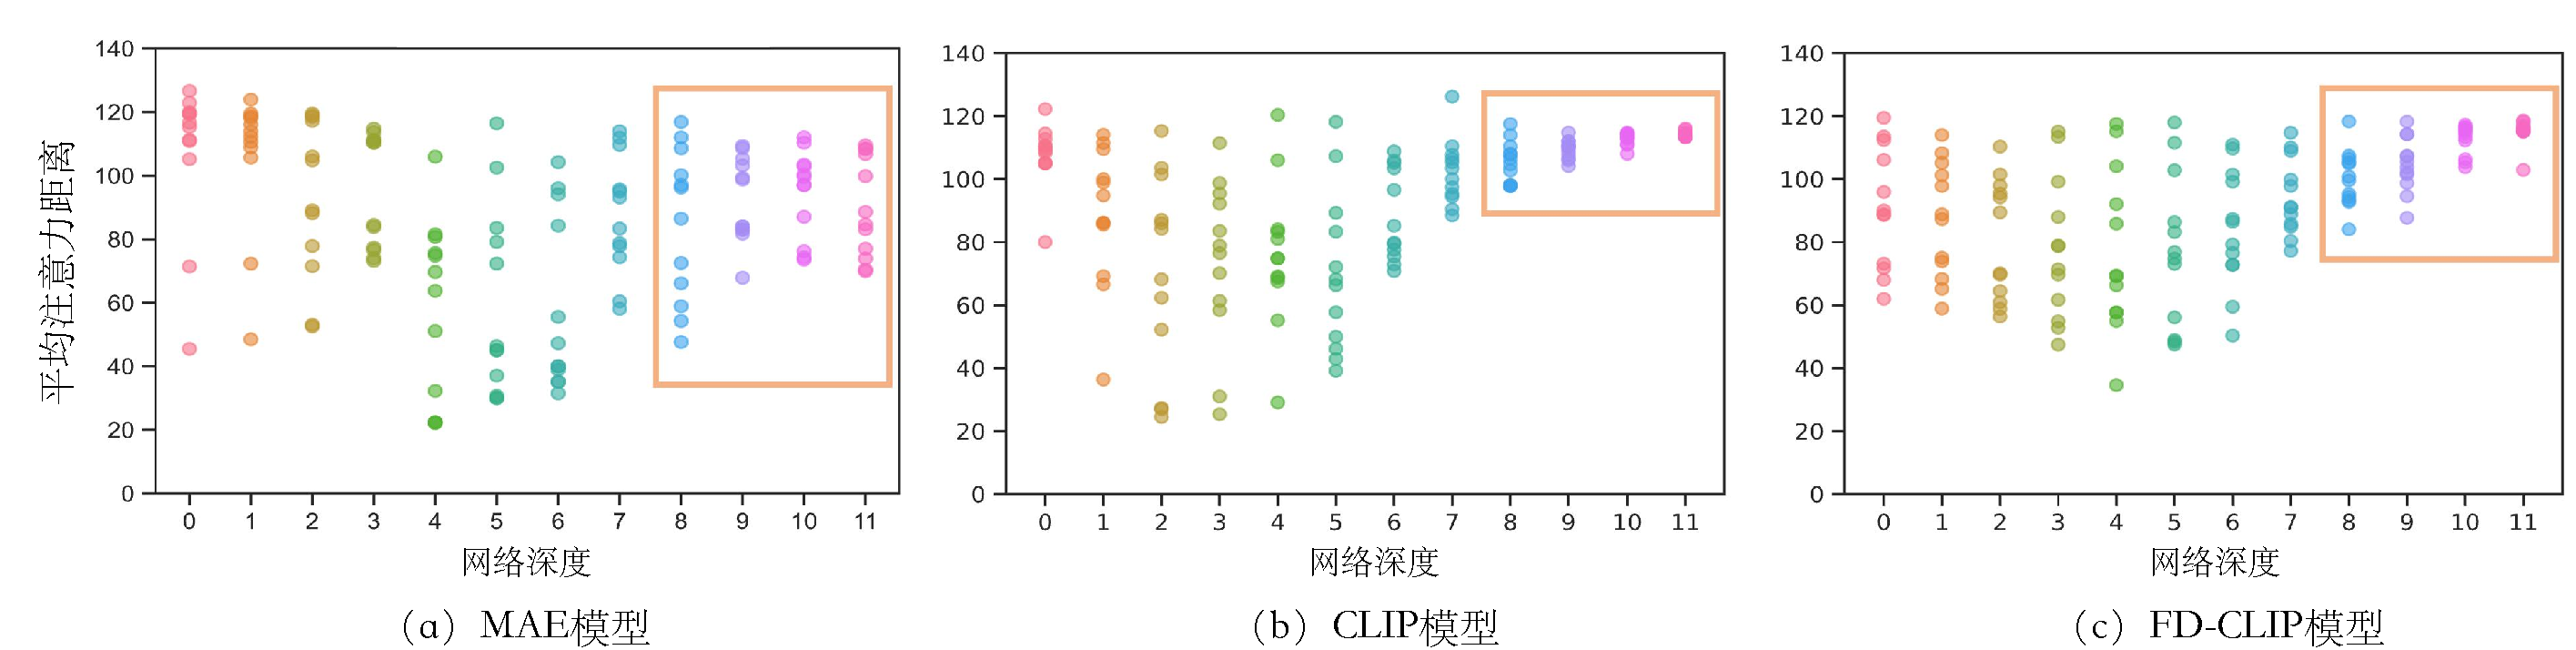
\includegraphics[width=1.0\linewidth]{figures/fd-attn-distance.pdf}
  \caption{不同预训练方法模型的平均注意力距离分布}
  \label{fig:fd-attn-distance}
\end{figure}
\paragraph{感受野多样化的注意力头} 首先使用注意力头级别的诊断工具分析了模型不同注意头的图像感受野多样性。图\ref{fig:fd-attn-distance}分别展示了MAE模型、原始CLIP模型和经过特征图自蒸馏后的FD-CLIP模型中不同网络深度的模型层内每个注意力头的平均注意力距离。
可以看到,在所有模型中,深度较浅的模型层里不同注意力头的感受野范围比较发散,说明此时模型既能建模局部的图像信息,又能获取全局的图像信息,展现了注意力头间的多样性。
然而,这种感受野的多样性在原始CLIP模型的较深模型层中迅速缩减。这表明模型的表达能力没有得到充分利用\cite{xie2023revealing}。
相比之下,FD-CLIP模型缓解了这个问题。FD-CLIP模型不同注意力头的感受野多样性在较深的模型层中保留得更好,也与掩码图像模型MAE方法的模型特征更为相似。%,表明它的模型容量可能被利用地更好。

\begin{figure}
  \centering
  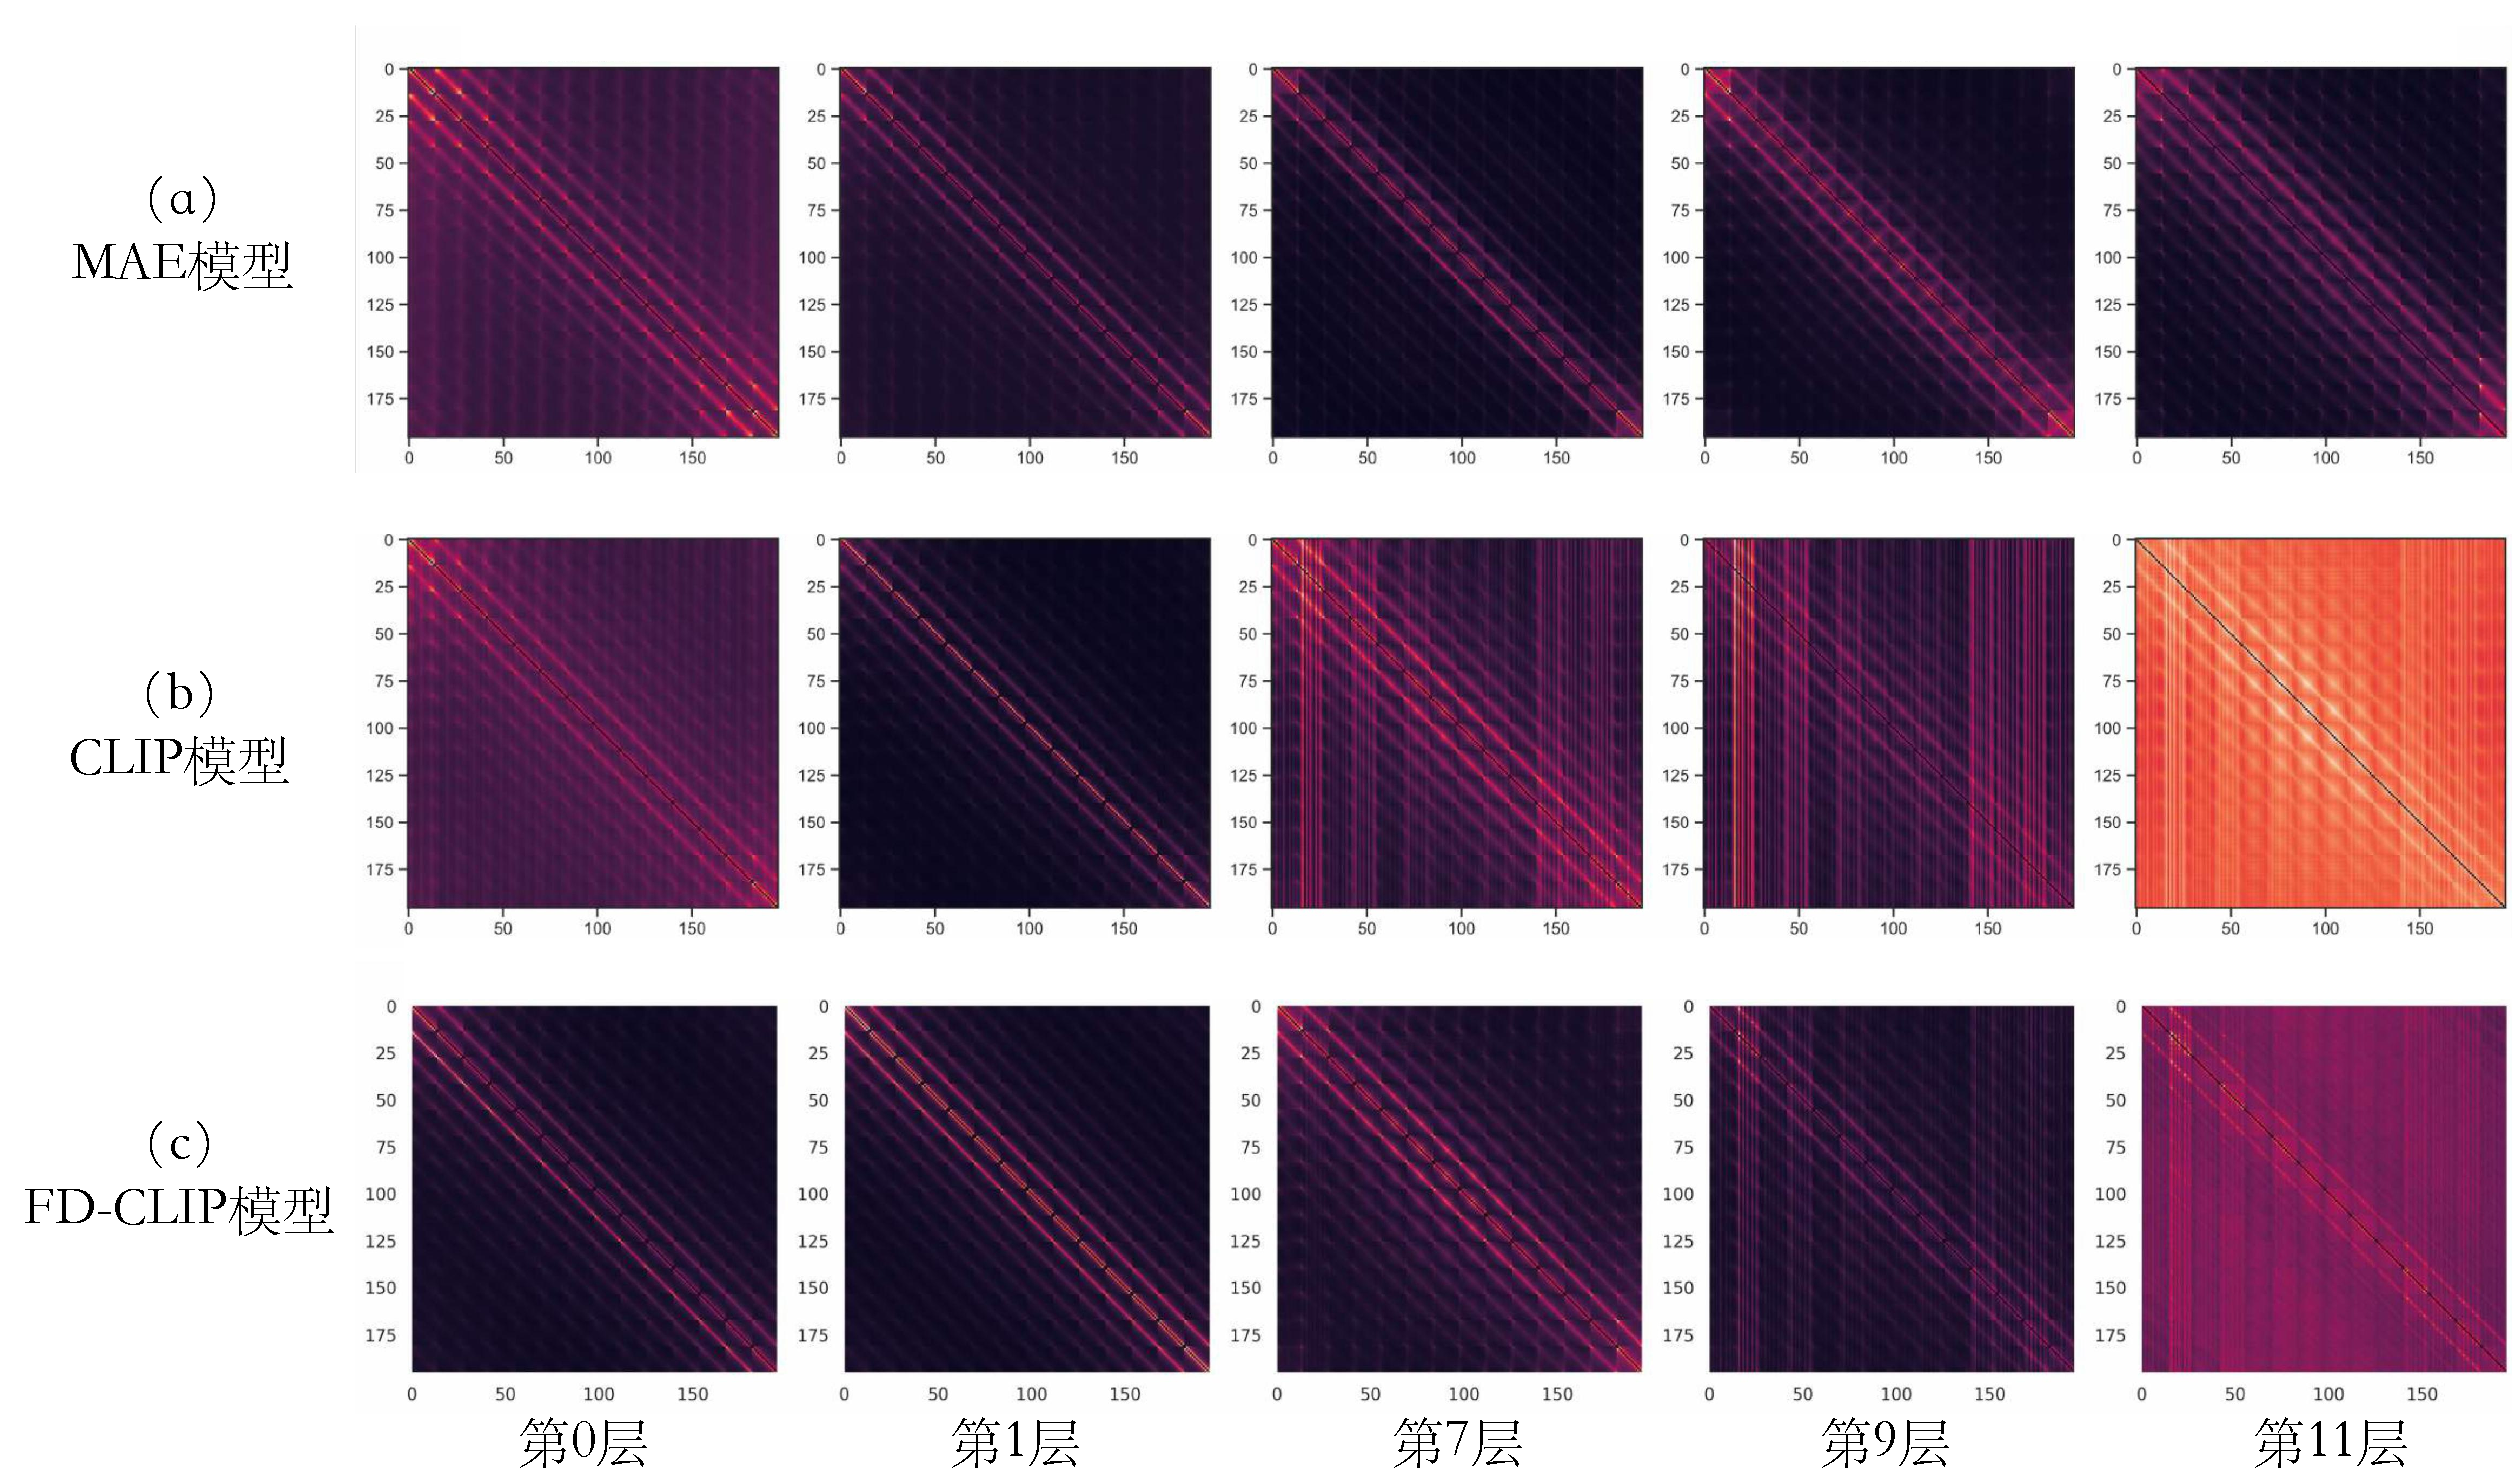
\includegraphics[width=1.0\linewidth]{figures/fd-attn-map.pdf}
  \caption{不同预训练方法模型的平均注意力图表现}
  \label{fig:fd-attn-map}
\end{figure}

\paragraph{平移不变性增强的注意力图} 图\ref{fig:fd-attn-map}展示了不同模型中某一层的平均注意力图。与原始CLIP模型相比,MAE模型的平均注意力图显示出更多的对角线模式,表明其更注重来自相对位置的视觉信息。这种特征属性表明掩码图像模型方法可以驱使模型学习到更强的图像表征平移不变性。这种局部敏感性使得模型在需要密集感知能力的细粒度下游任务上有更好的微调表现。
而CLIP模型在更深的层(7至11层)中展现出了更多垂直模式,这表明CLIP模型的图像表征被一些处于绝对位置的输入像素主导。经过特征图自蒸馏方法之后,FD-CLIP模型的平均注意力图中垂直模式部分消失,图像表征的平移不变性得到增强,与掩码图像模型MAE方法的模型特征更为相似,因此有助于提高下游任务迁移性能。

\begin{figure}
  \centering
  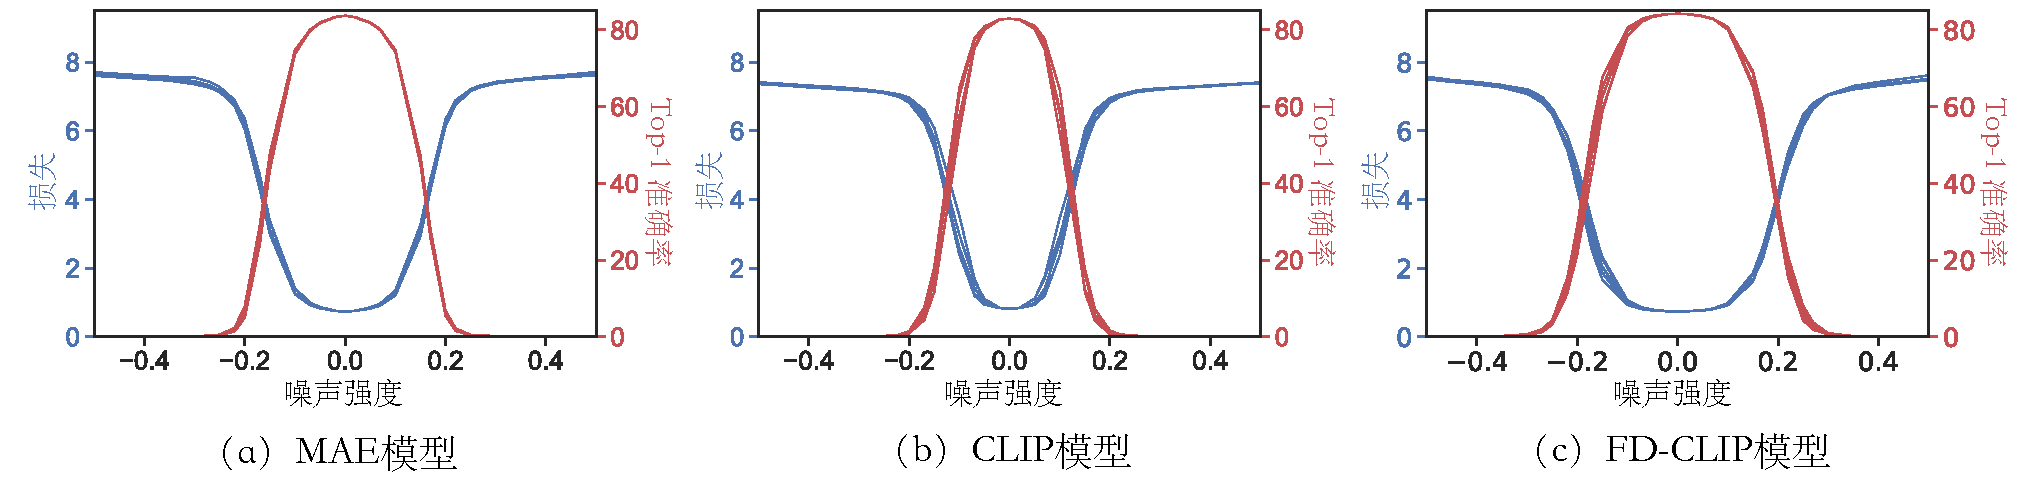
\includegraphics[width=1.0\linewidth]{figures/fd-loss-landscape.pdf}
  \caption{不同预训练方法模型的损失景观和准确率景观}
  \label{fig:fd-loss-landscape}
\end{figure}

\paragraph{损失景观的扁平化} 图\ref{fig:fd-loss-landscape}显示了不同模型在不同噪声强度影响下的损失景观和准确率景观\cite{li2018visualizing}。从可视化结果中可以看出,MAE模型和FD-CLIP模型的损失景观相比于原始CLIP模型的损失景观更加平坦,表明了经过特征图自蒸馏后的模型在下游视觉任务的优化过程更加平稳,泛化性能更好。% 这一观察结果也与它在实验中更好的微调效果一致。

% 图 3:(a) MAE [17]、(b) CLIP [42] 和 (c) FD-CLIP 上每个头部在每一层深度的平均注意力距离。距离是在像素级别测量的。

% 图 4:(a) MAE [17]、(b) CLIP [42] 和 (c) FD-CLIP 上的平均注意力图。这些地图是所有头部和所有图像的平均值。选择五个代表性图层,即第 0、1、7、9、11 个图层,以节省空间。完整的注意力地图可以在补充材料中找到。

% 图5:(a)平均绝对误差(MAE)[17]、(b)对比语言-图像预训练(CLIP)[42] 以及(c)FD - CLIP的损失/准确率态势图[33],其中x轴表示噪声强度,y轴表示损失/准确率。每张图展示了使用5个随机生成方向得到的5个态势图。 

\begin{figure}
  \centering
  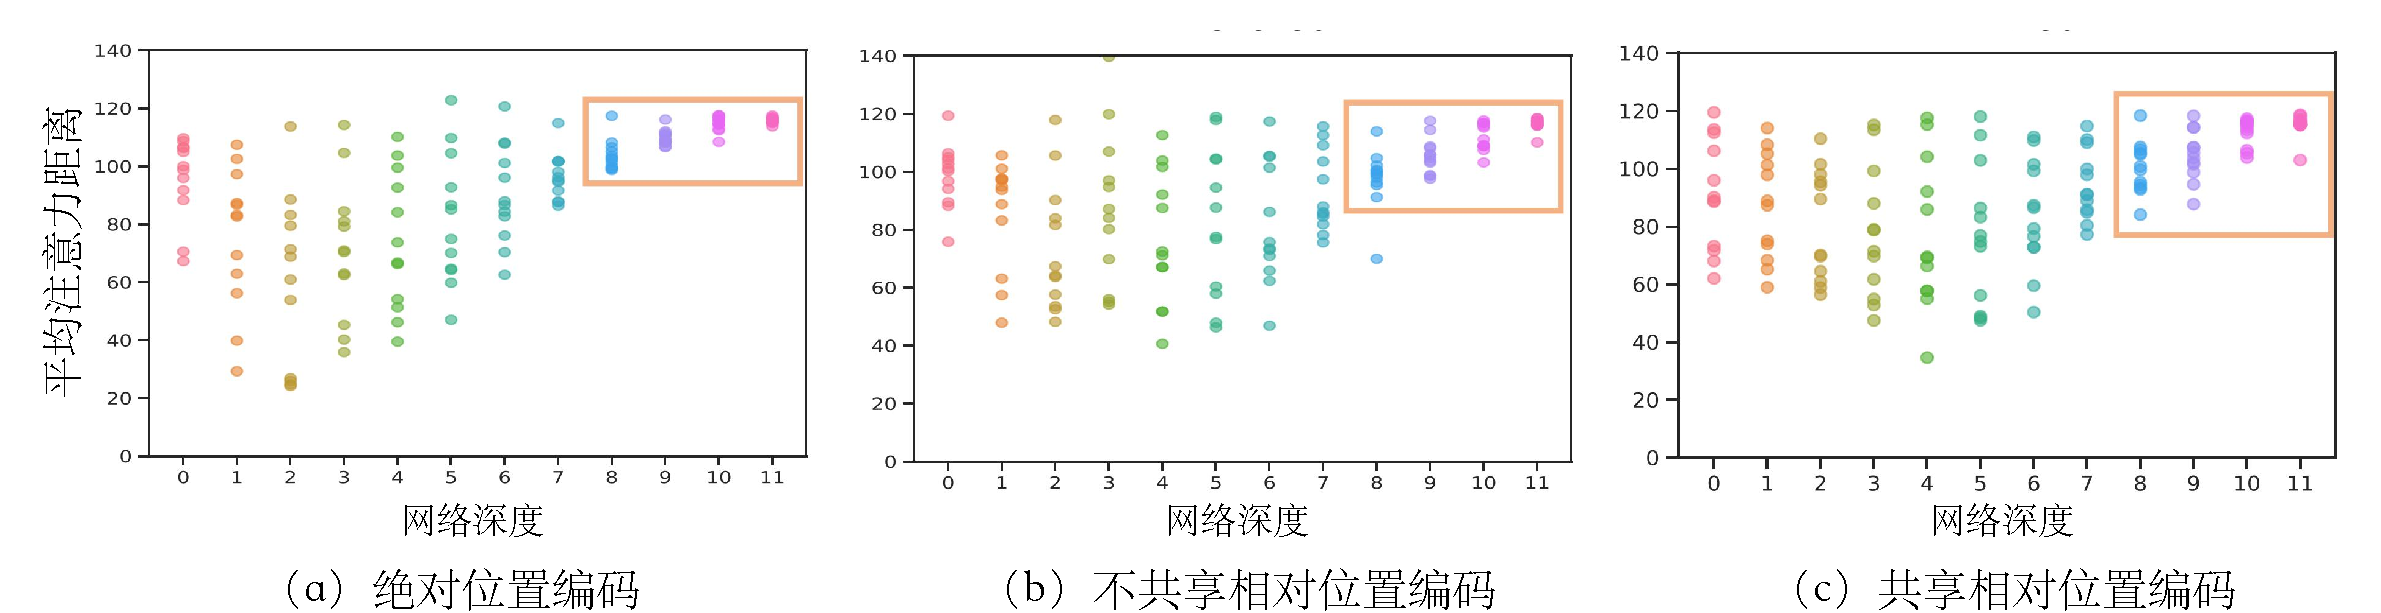
\includegraphics[width=1.0\linewidth]{figures/fd_compare_all_ape_rpe.pdf}
  \caption{层间共享的相对位置编码提升了模型注意力头的多样性}
  \label{fig:fd_compare_all_ape_rpe}
\end{figure}

\paragraph{位置编码策略对注意力头多样性的影响} 特征图自蒸馏方法在学生模型中引入了层间共享的相对位置编码设计,以减少在较深的模型层中出现不同像素表征间过于相似的现象。表\ref{tab:fd-ablation_tricks}(c)中的消融实验结果表明这种归纳偏置对CLIP模型的迁移性能有改进作用。
本节分析了在特征图自蒸馏过程使用不同位置编码配置的模型特征属性区别,包括绝对位置编码、不共享相对位置编码和共享相对位置编码。图\ref{fig:fd_compare_all_ape_rpe}中展示了在使用不同位置编码配置的情况下模型各注意力头的平均注意力距离分布。
与使用绝对位置编码和不共享相对位置编码的模型相比,使用共享相对位置编码的模型在更深的模型层中注意力头的感受野大小更加多样化,表明此时模型深层参数的冗余性更低。这一观察解释了这种共享相对位置编码具有更佳迁移效果的原因。


\section{总结}
\label{sec:fd-summary}


% CLIP 模型已经展示了令人印象深刻的高零镜头识别精度,但是,它们在下游视觉任务上的迁移性能并不理想。相反,尽管在训练过程中没有语义标签,但掩码图像模型 (MIM) 在对下游任务的微调方面表现异常出色。我们注意到这两个任务具有不同的成分:图像级目标与标记级目标,交叉熵损失与回归损失,以及全图像输入与部分图像输入。为了减少差异,我们引入了一个经典的特征图蒸馏框架,它可以同时保留 CLIP 模型的语义能力,同时构建一个包含 MIM 关键成分的任务。实验表明,特征图蒸馏方法显著提高了 CLIP 模型在几个典型的下游视觉任务上的迁移性能。我们还观察到该方法产生了新的 CLIP 表示,这些表示与 MIM 的表示具有一些共享的诊断特性。此外,特征图蒸馏方法推广到其他预训练模型,如 DINO、DeiT 和 SwinV2-G,在 MSCOCO 对象检测方面达到了 64.2 mAP 的新纪录,提高了 +1.1。

% 我们的贡献总结如下:
% ・我们研究了 CLIP 和 MIM 方法之间的成分差异,并证明靶标粒度对于 MIM 在微调中的成功至关重要。
% ・我们利用经典的特征图蒸馏将 CLIP 的训练目标粒度转换为令牌级的粒度,从而增强了其 performance 并保留其语义信息。
% ・我们在特征蒸馏过程中提出了几种进一步扩大改进的关键技术,包括蒸馏标准化特征图、不对称滴路径速率和共享相对位置偏置。
% ・通过多种诊断工具,我们发现与 CLIP 相比,MIM 和 FD-CLIP 都具有几个直观上良好的特性,这可能为它们卓越的迁移性能提供见解。
% ・我们将我们的方法推广到各种预训练模型,并观察到一致的收益。我们还通过使用我们的框架改进先进的 3B SwinV2-G 模型,创造了 MSCOCO 对象检测的新记录。

% 背景+motivation
语言-图像对比学习方法利用大规模图文对数据学习了丰富的语义信息,在零样本开放集合图像识别任务上表现优异。然而,CLIP模型在许多下游视觉任务,尤其是依赖密集感知能力的细粒度视觉任务上的迁移表现不佳。
% 前一章中提出的iCLIP方法通过引入已有的低噪声有标注数据,有效地扩展了CLIP模型训练可利用数据源的同时,显著提高了数据利用的效率。但这种方法得到的CLIP模型在迁移到下游视觉任务,尤其是细粒度视觉任务上的性能提升有限。
% 语言-图像对比学习方法利用大规模图文对数据学习了丰富的语义信息,因此在固定视觉模型只微调分类器的线性探测任务上可以取得非常优异的表现。然而,相比于像素级自监督方法,语言-图像对比学习方法得到的视觉模型在许多下游视觉任务,尤其是依赖密集感知能力的细粒度视觉任务上的迁移性能并无优势。

% 解决方案和发现
本章提出将掩码图像模型的像素级训练目标引入语言-图像对比学习方法中。为避免人工标注大规模图文对数据,同时无须重新预训练CLIP模型,本章提出特征图自蒸馏微调方法。
特征图自蒸馏方法通过CLIP模型自身作为教师模型,提取输出特征图作为重新初始化的学生模型的训练目标。这种方法一方面无需额外标注即可构造像素级训练目标,另一方面以较低代价将教师模型的预训练知识转移到学生模型中。
此外,本章还提出多种模型特征属性诊断工具对自蒸馏前后的模型进行分析,并揭示了自蒸馏后的模型与掩码图像模型具有一些相似性质,解释了特征图自蒸馏方法的有效性。
经过特征图自蒸馏后的CLIP模型在语义分割、目标检测、深度估计等细粒度下游视觉任务上取得明显性能提升。进一步将该方法推广到有30亿参数的SwinV2-G模型后,取得了MSCOCO数据集上目标检测任务的新纪录。
% 实验观察到像素级图像自监督预训练模型,如掩码图像模型(MIM),在下游任务上的迁移表现优异。受该类方法启发,本章仔细研究了两种不同预训练任务的建模区别,并着重讨论了输入图像完整性和训练目标粒度对视觉任务迁移性能的影响。
% 为低代价地在CLIP模型中引入像素级训练目标,同时避免大规模的数据标注以利用互联网级数据,本章提出使用特征图自蒸馏的方法,在尽可能保留CLIP模型中蕴含的语义信息同时引入像素级的监督目标。这种方法无须重新训练CLIP模型,且相比于原本CLIP模型训练代价而言,只需要额外3\%的训练成本即可显著提升其在各类下游任务,尤其是细粒度视觉任务上的性能表现。
% 通过在特征图自蒸馏框架中设计不同训练目标粒度和不同输入图像比例的实验,结果表明提升下游任务迁移性能的关键在于应用像素级的训练目标粒度。
% 此外,本章还提出利用多种注意力头级、模型层级、模型级的诊断工具对自蒸馏前后的模型进行分析和理解,可视化观察显示经过特征图自蒸馏的FD-CLIP在直观上拥有一些和MIM模型类似的特性,这为它们优异的迁移性能提供了见解。
% 为进一步验证该框架的通用性和可扩展性,本章将该框架用于不同视觉模型结构、不同预训练任务和不同模型规模的视觉模型,并观察到一致的收益。通过特征图自蒸馏框架改进的有30亿参数的SwinV2-G模型,创造了当时MSCOCO数据集上目标检测的新纪录。

% 引出下一章
虽然本章工作研究了提升语言-图像对比学习方法在下游视觉任务上迁移性能的方法,但其在语义生成任务上的迁移方式仍待探索。下一章以图像描述生成任务为主要场景,研究了语言-图像对比学习方法在语义生成任务上的迁移方法。